%!TEX root = main.tex
In a practical application, the emitter and receiver do not share the same physical location and use local oscillators.
For this reason, the communication is affected by different effects: CFO and SCO due to the imperfections of the crystals, carrier phase error and sample time shift due to the fact that the oscillators are not physically the same.
The baseband model of the effects of these imperfections is presented on figure~\ref{fig:sync}.
\begin{figure}[htbp]
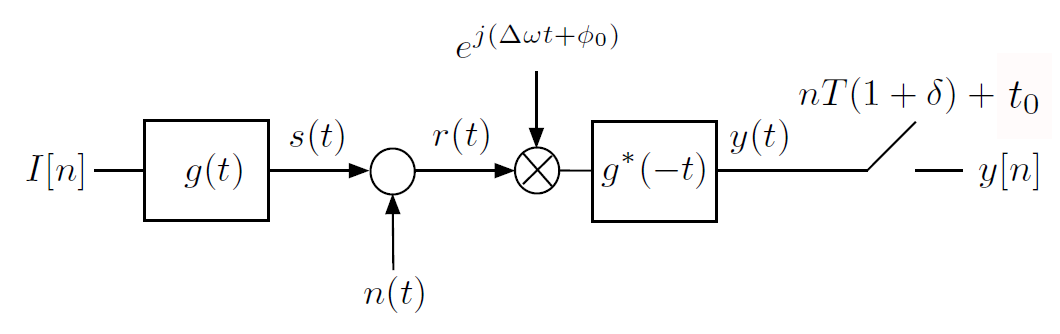
\includegraphics[width=\textwidth]{baseband_sync.png}
\caption[Baseband model with synchronization errors.]{Baseband model with synchronization errors. [Source: course notes]\label{fig:sync}}
\end{figure}

In this section, we will implement estimation and compensation algorithms for the sample time shift and the CFO, then assess their performances.
\subsection{Effect of the CFO-caused ISI on the BER}
The degradation of the BER due only to the ISI introduced by the CFO is shown in figure~\ref{fig:cfoisiber}.
\begin{figure}[htbp]
\centering
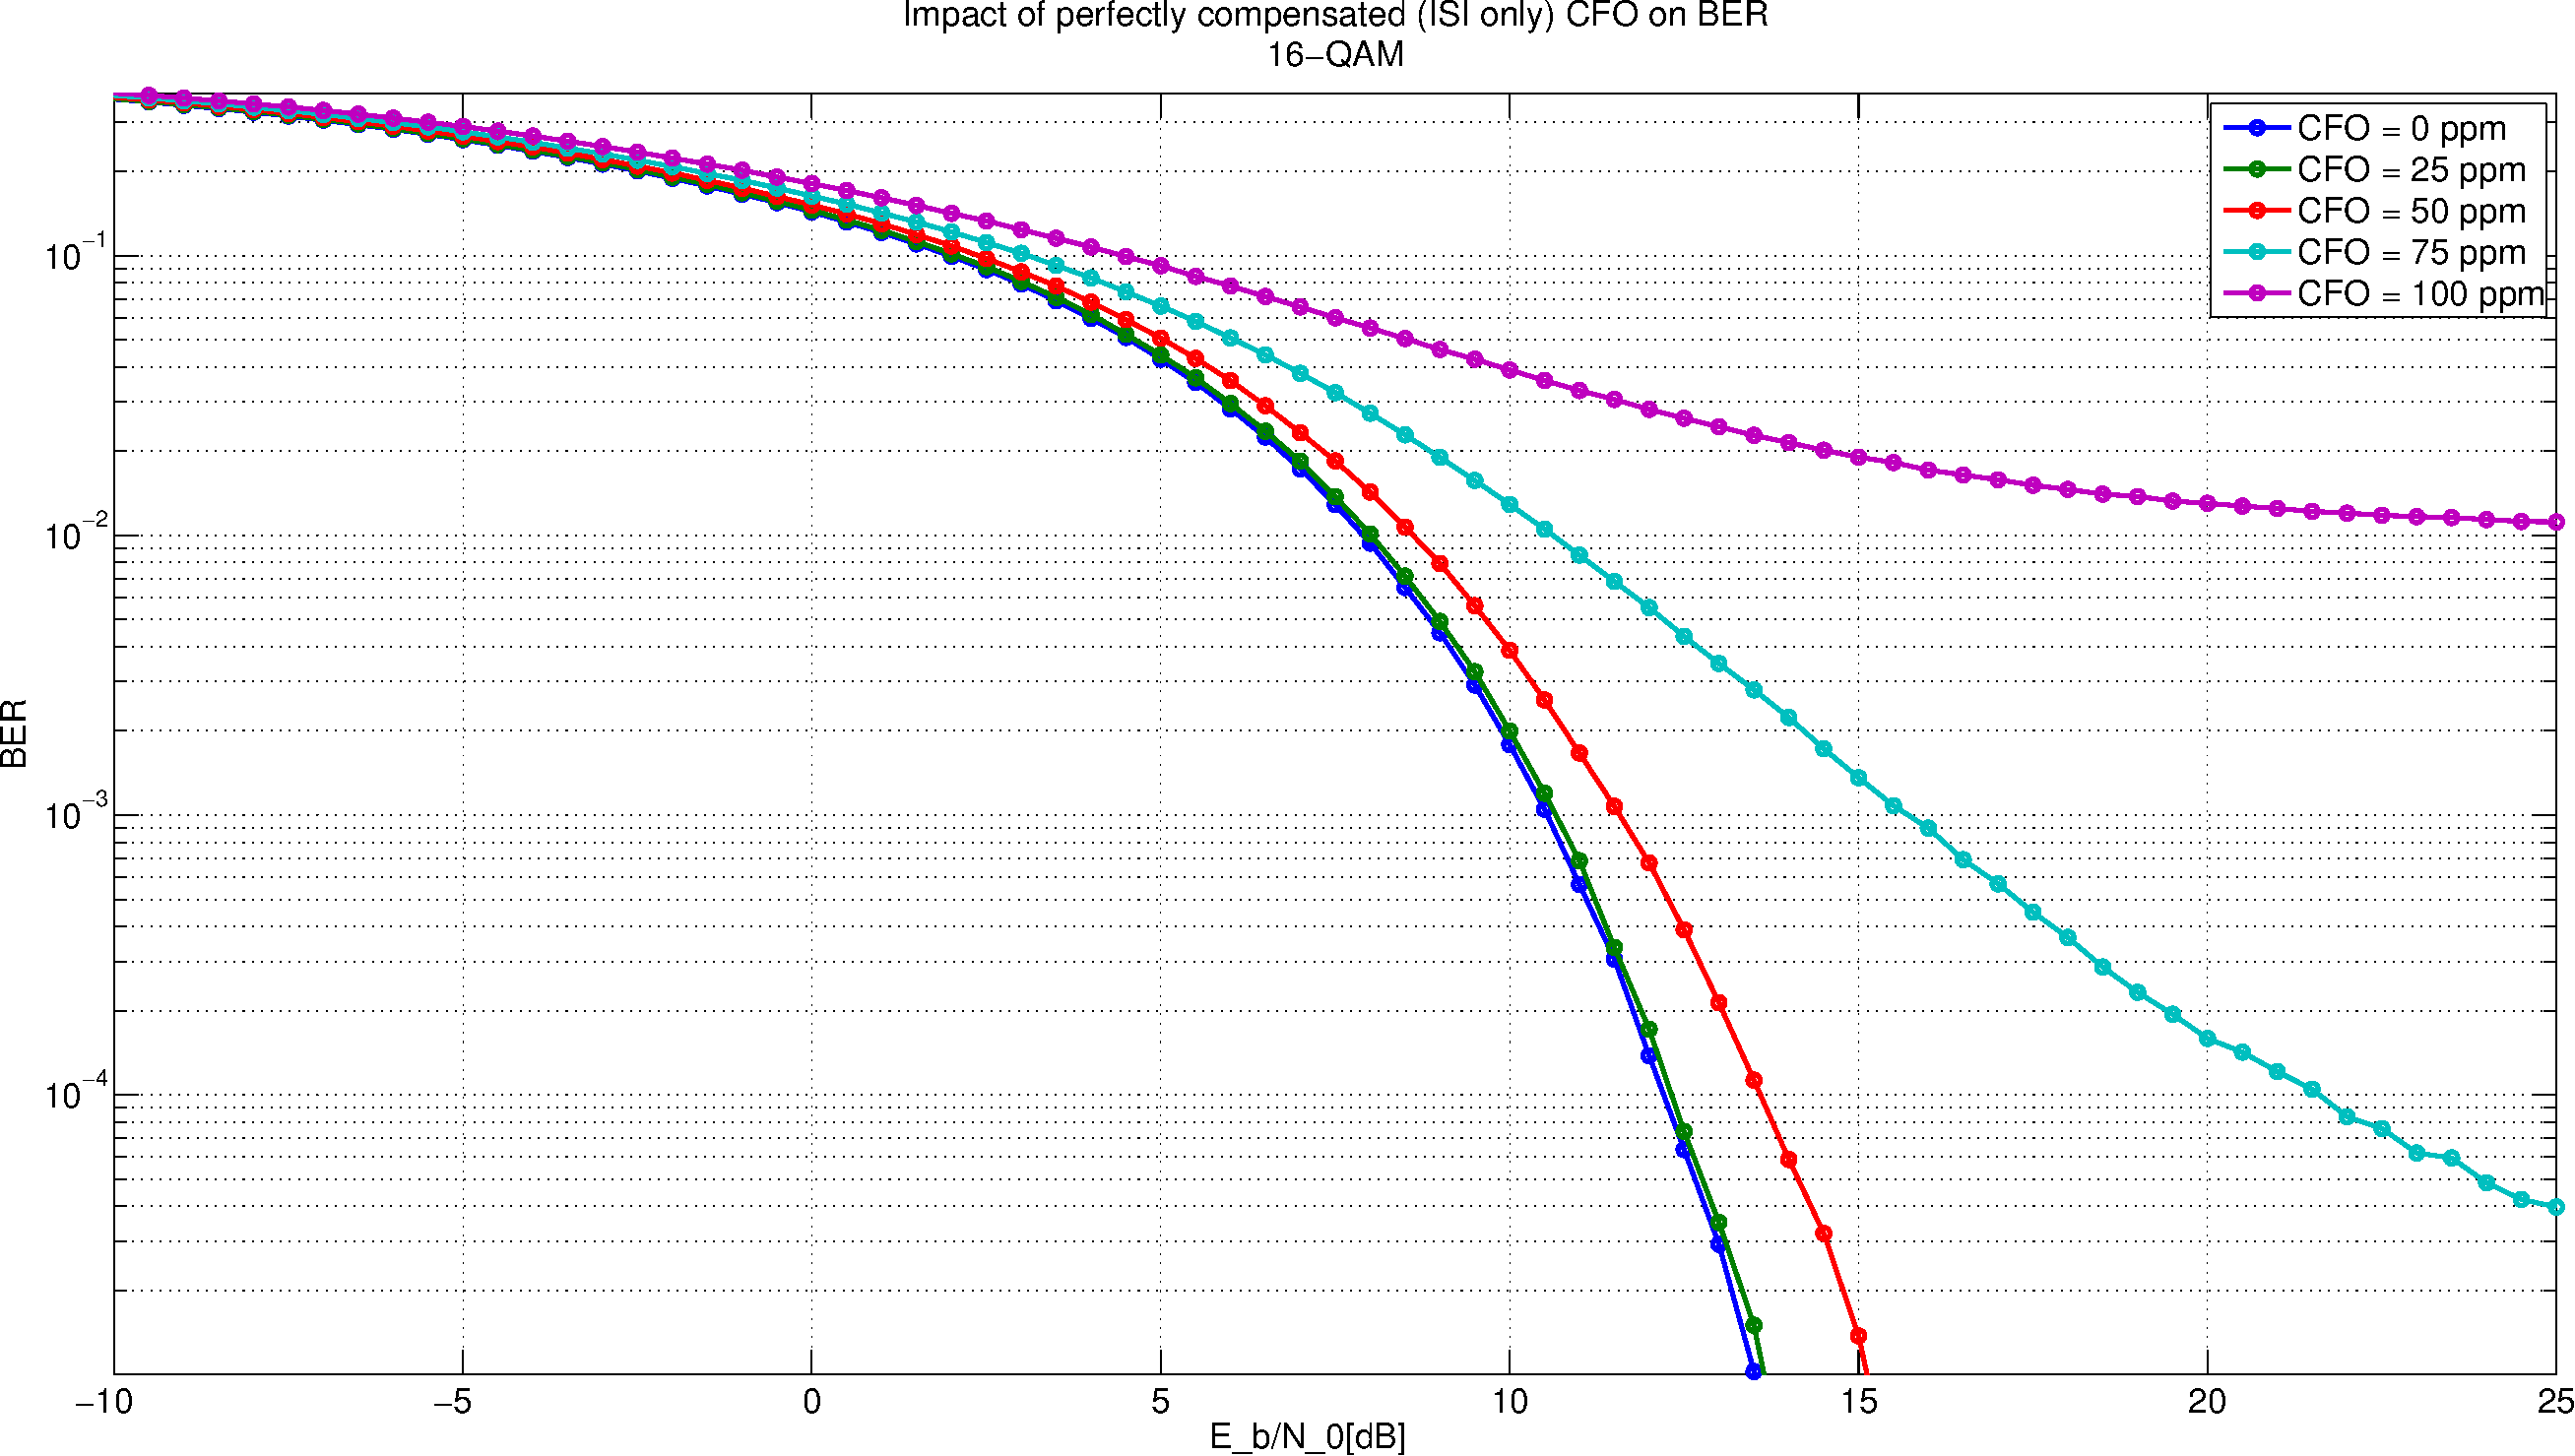
\includegraphics[width=\textwidth]{cfoisiber.pdf}
\caption{Impact of the ISI introduced by the CFO on the BER.\label{fig:cfoisiber}}
\end{figure}
Figure~\ref{fig:cfoisiber} shows that for a given value of $\Delta\omega$ and at higher noise levels, the BER curve is worsened but shows similar behaviour as the original curve with no CFO.
However, past a certain value of $\frac{E_b}{N_0}$, the BER stops decreasing and only the errors introduced by the ISI subsist.
Those plateaus in the curves correspond to what we observed when we were testing the simulation with no CFO but with a badly defined pair of nyquist filters which did not sufficiently cancel the ISI.

To conclude, figure~\ref{fig:cfoisi} shows the ISI of two halfroot nyquist filters separated by CFO.
\begin{figure}[htbp]
    \centering
    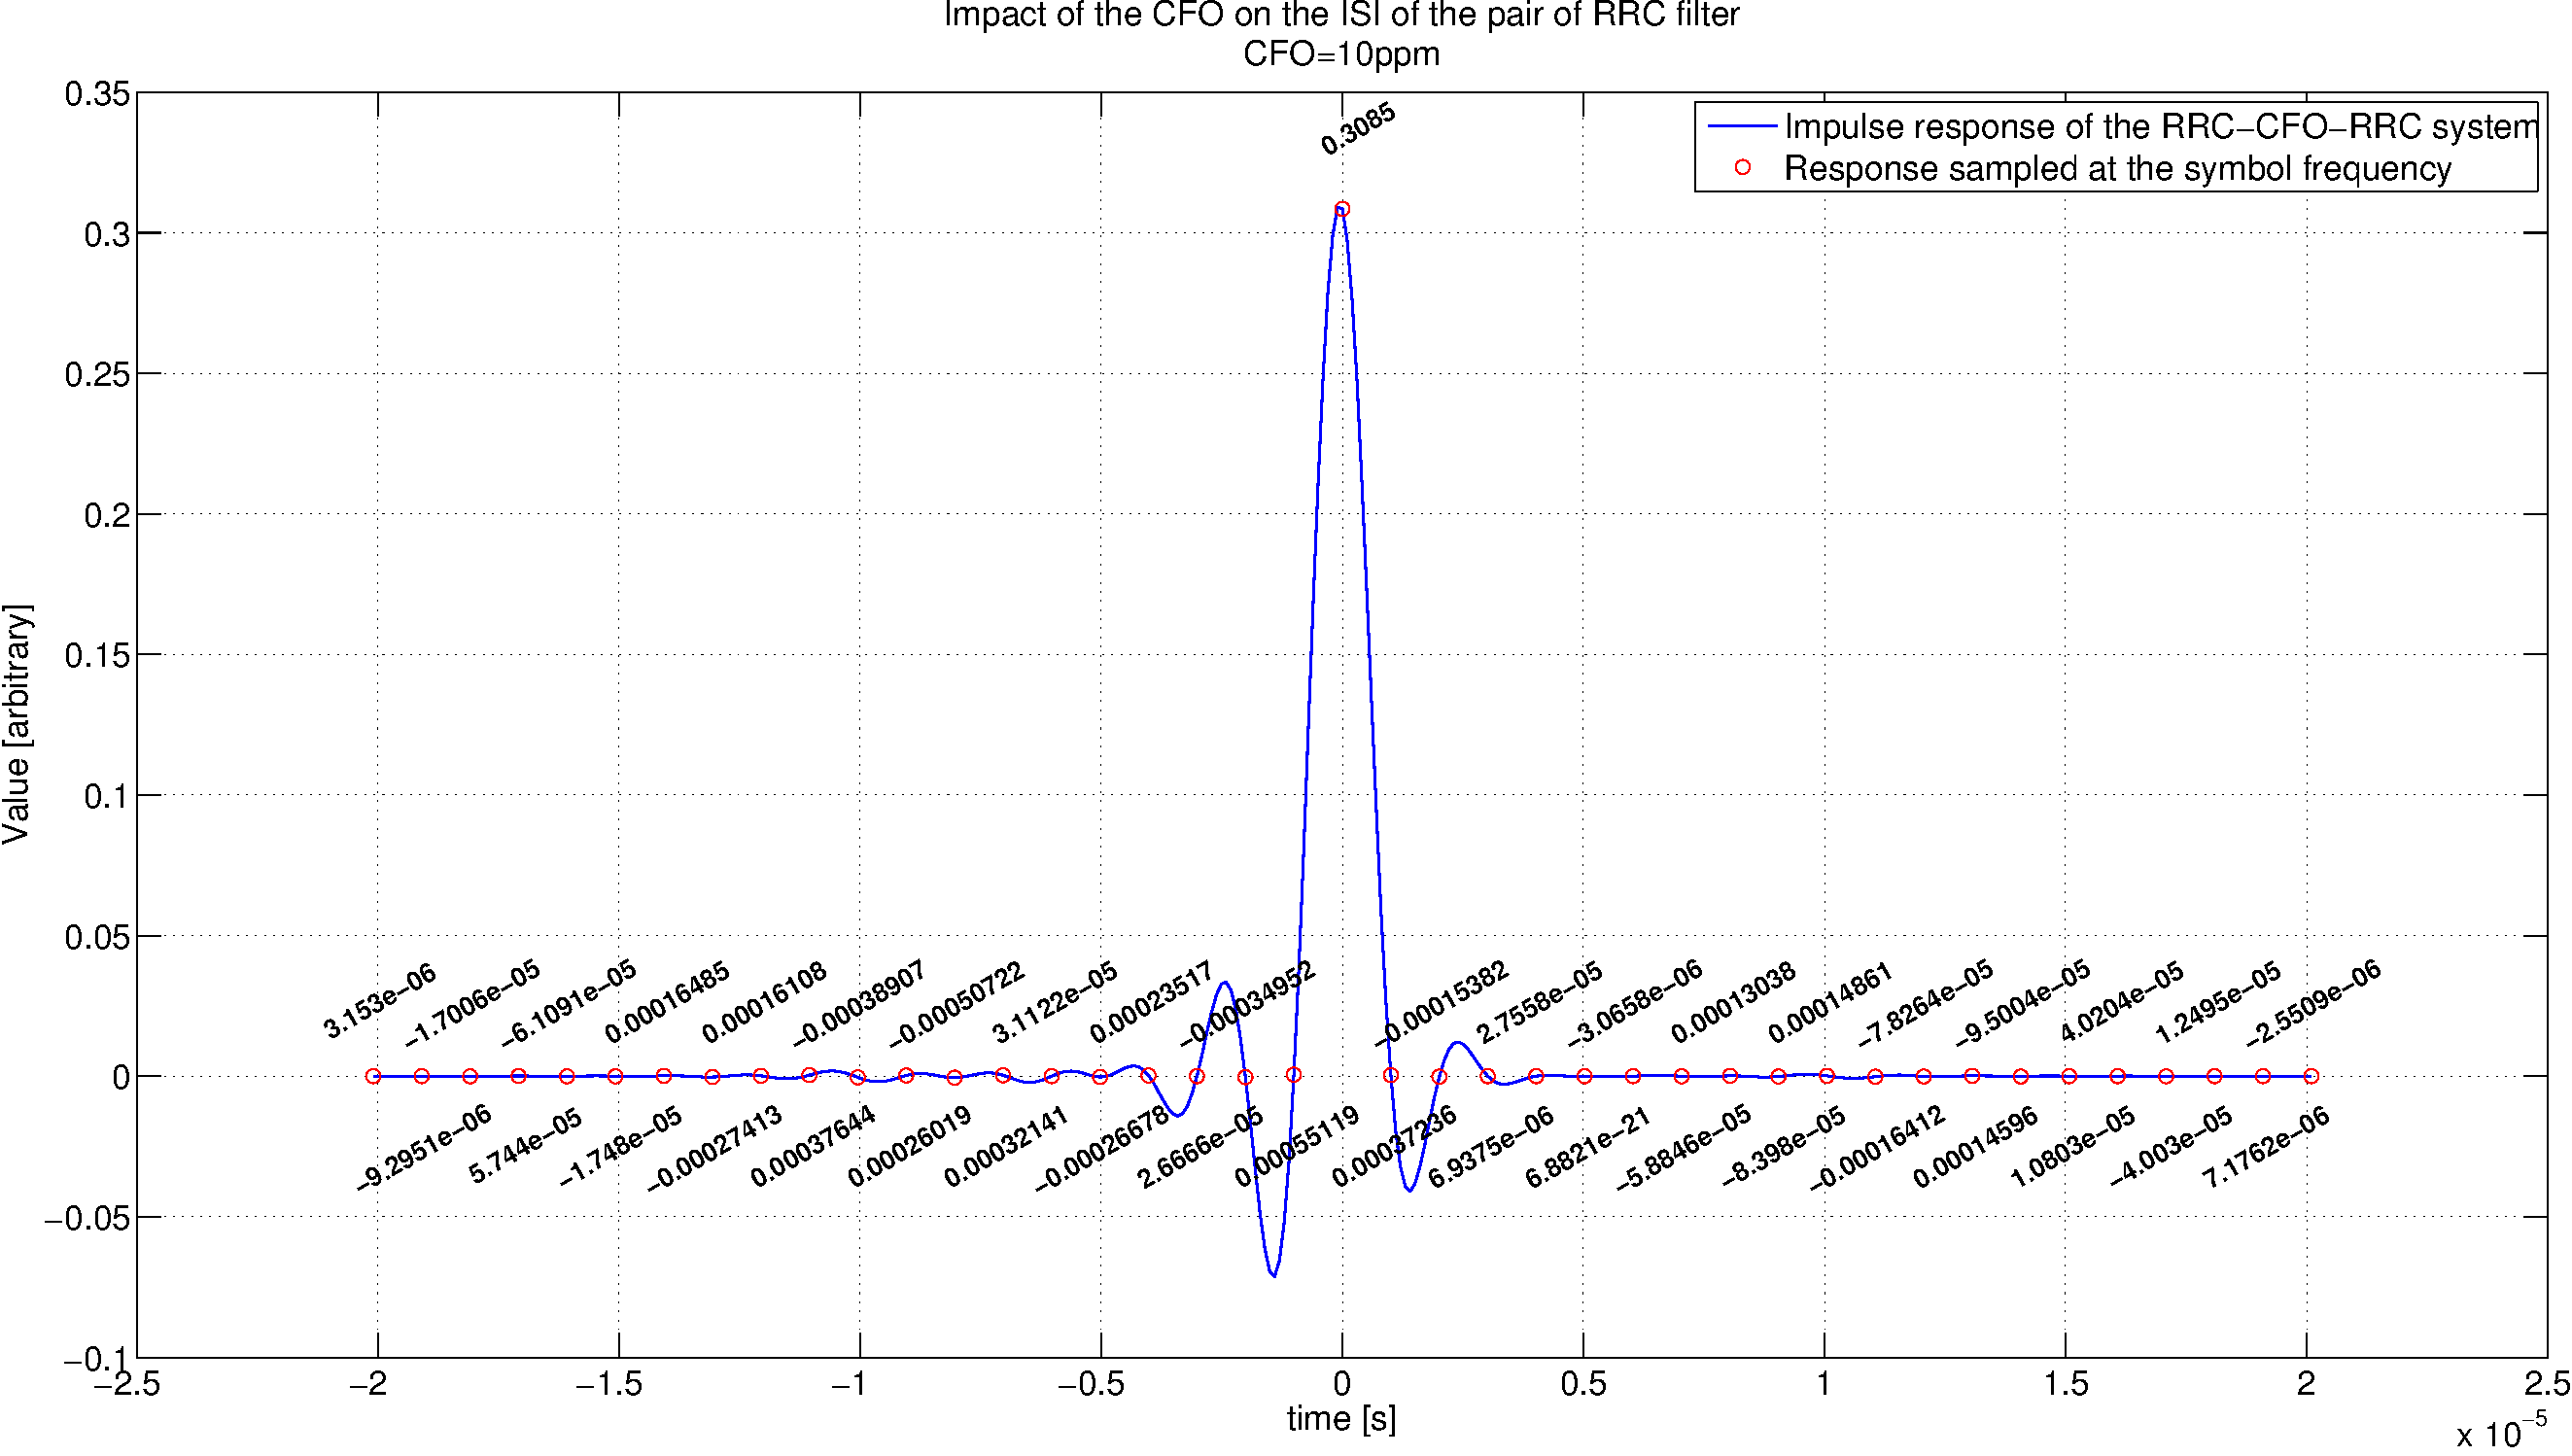
\includegraphics[width=\textwidth]{cfoisi.pdf}
    \caption[Effect of \SI{10}{ppm} of CFO on the ISI of the pair of filters.]{Effect of \SI{10}{ppm} of CFO on the ISI of the pair of filters. $f_c = \SI{2}{\giga\hertz}$, $\Rightarrow \Delta\omega = \SI{20}{\kilo\hertz}$.\label{fig:cfoisi}}
\end{figure}

\subsection{Effect of uncompensated CFO on the BER}
If the CFO is not compensated, the slow phase drift over time renders the channel unusable and the BER is 0.5 at any noise level. Figure~\ref{fig:cfoconst} shows the effect of noise and CFO on the constellation. This helps understand how uncompensated CFO renders any communication impossible.
\begin{figure}
  \centering
  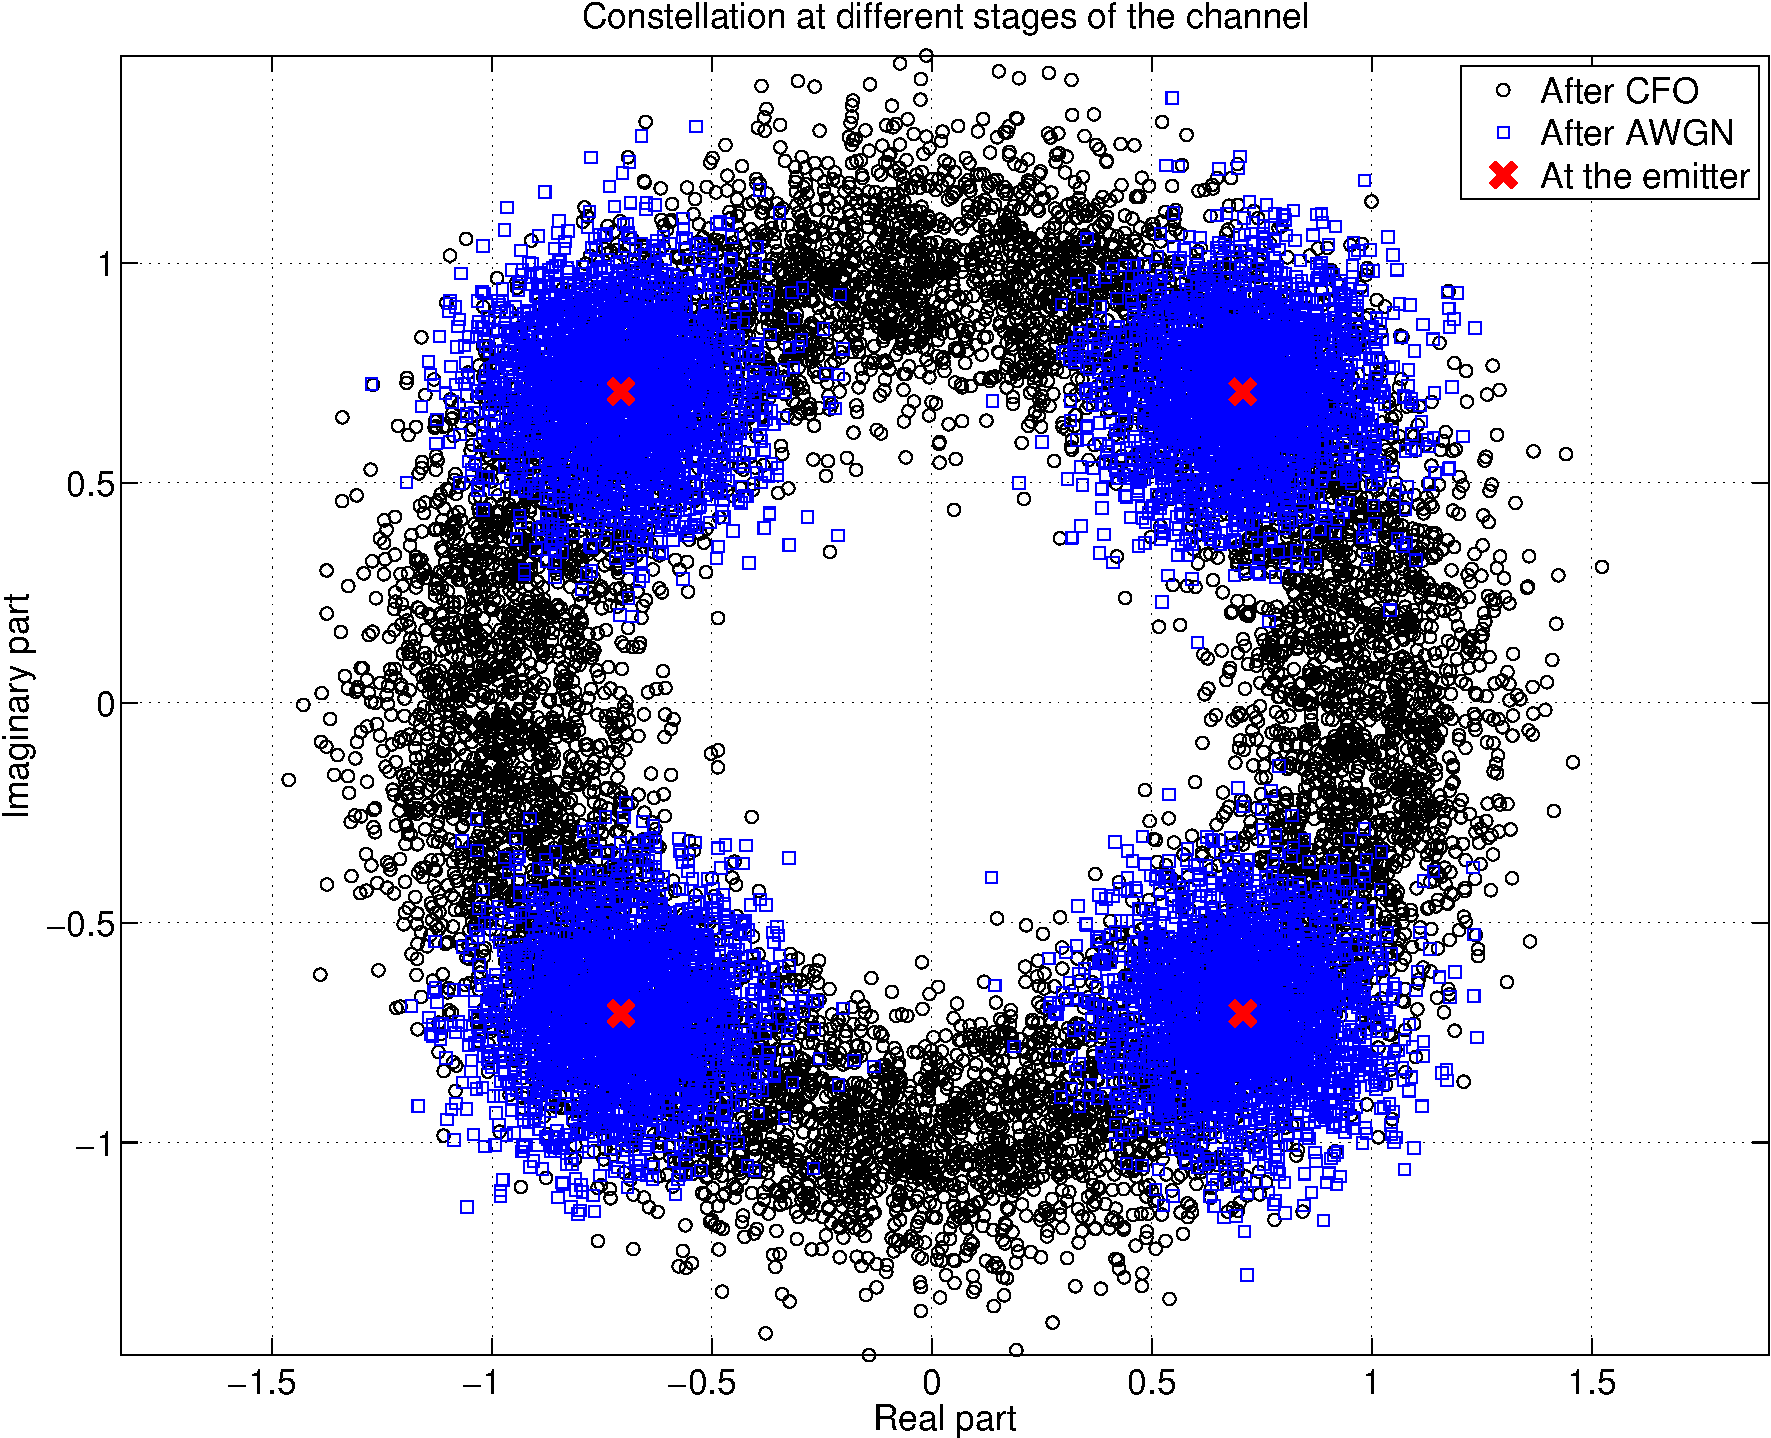
\includegraphics[width=.8\textwidth]{cfoconstellation.pdf}
  \caption[Constellation at different stages in the communication.]{Constellation at different stages in the communication. \SI{10}{ppm} of CFO, $f_c = \SI{2}{\giga\hertz}$, $\frac{E_b}{N_0} = \SI{10}{\decibel}$.\label{fig:cfoconst}}
\end{figure}

\subsection{Sample time shift error}
Figure~\ref{fig:smpEpsBER} shows the impact of the sample time shift on the error rate.
\begin{figure}[htbp]
\centering
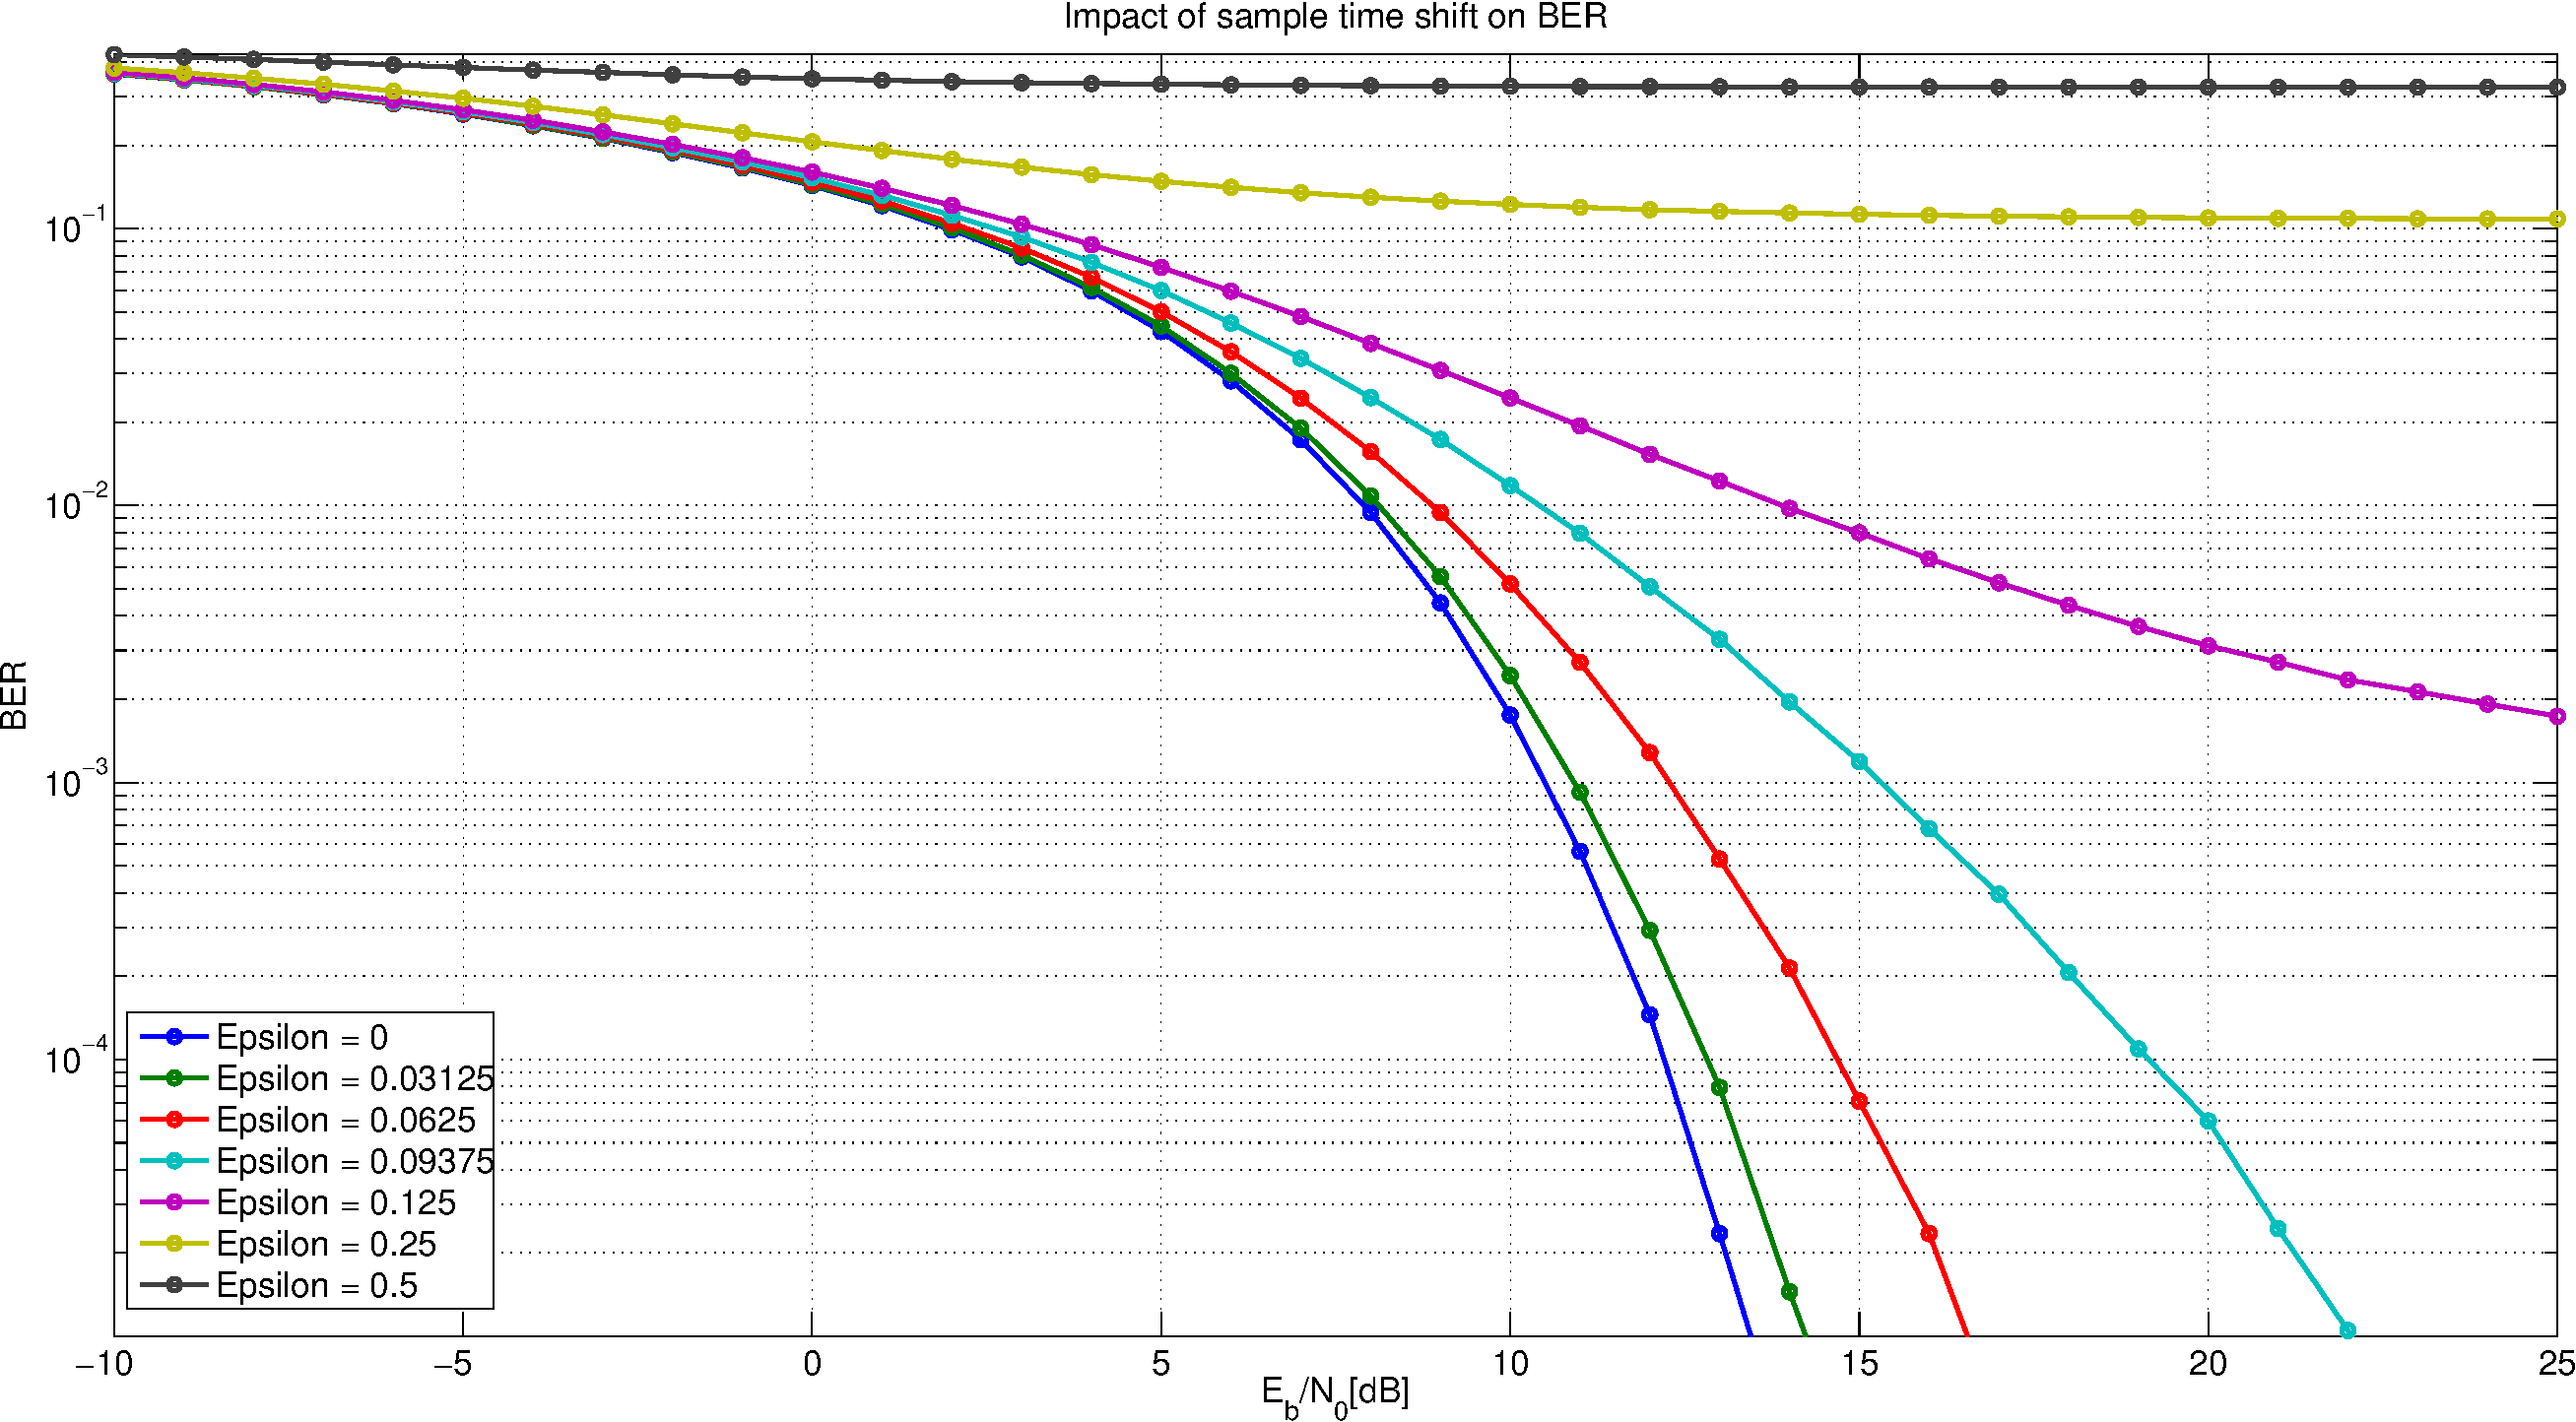
\includegraphics[width=\textwidth]{smpEpsBER.pdf}
\caption[Impact of the sample time shift on the error rate.]{Impact of the sample time shift on the error rate. $f_m = \SI{1}{\mega\hertz}$, $f_s = \SI{32}{\mega\hertz}$ $\Rightarrow \Delta k = 0, 1, 2, 3, 4, 8, 16$ samples.\label{fig:smpEpsBER}}
\end{figure}
As expected, the error rate is worsened by the sample time shift and the channel is unusable when the incoming signal is sampled exactly in between symbols.

\subsection{Sample time shift error correction using the Gardner Algorithm}
Figure~\ref{fig:gConvK} shows the convergence of the Gardner algorithm for different error weights.
\begin{figure}[htbp]
    \centering
    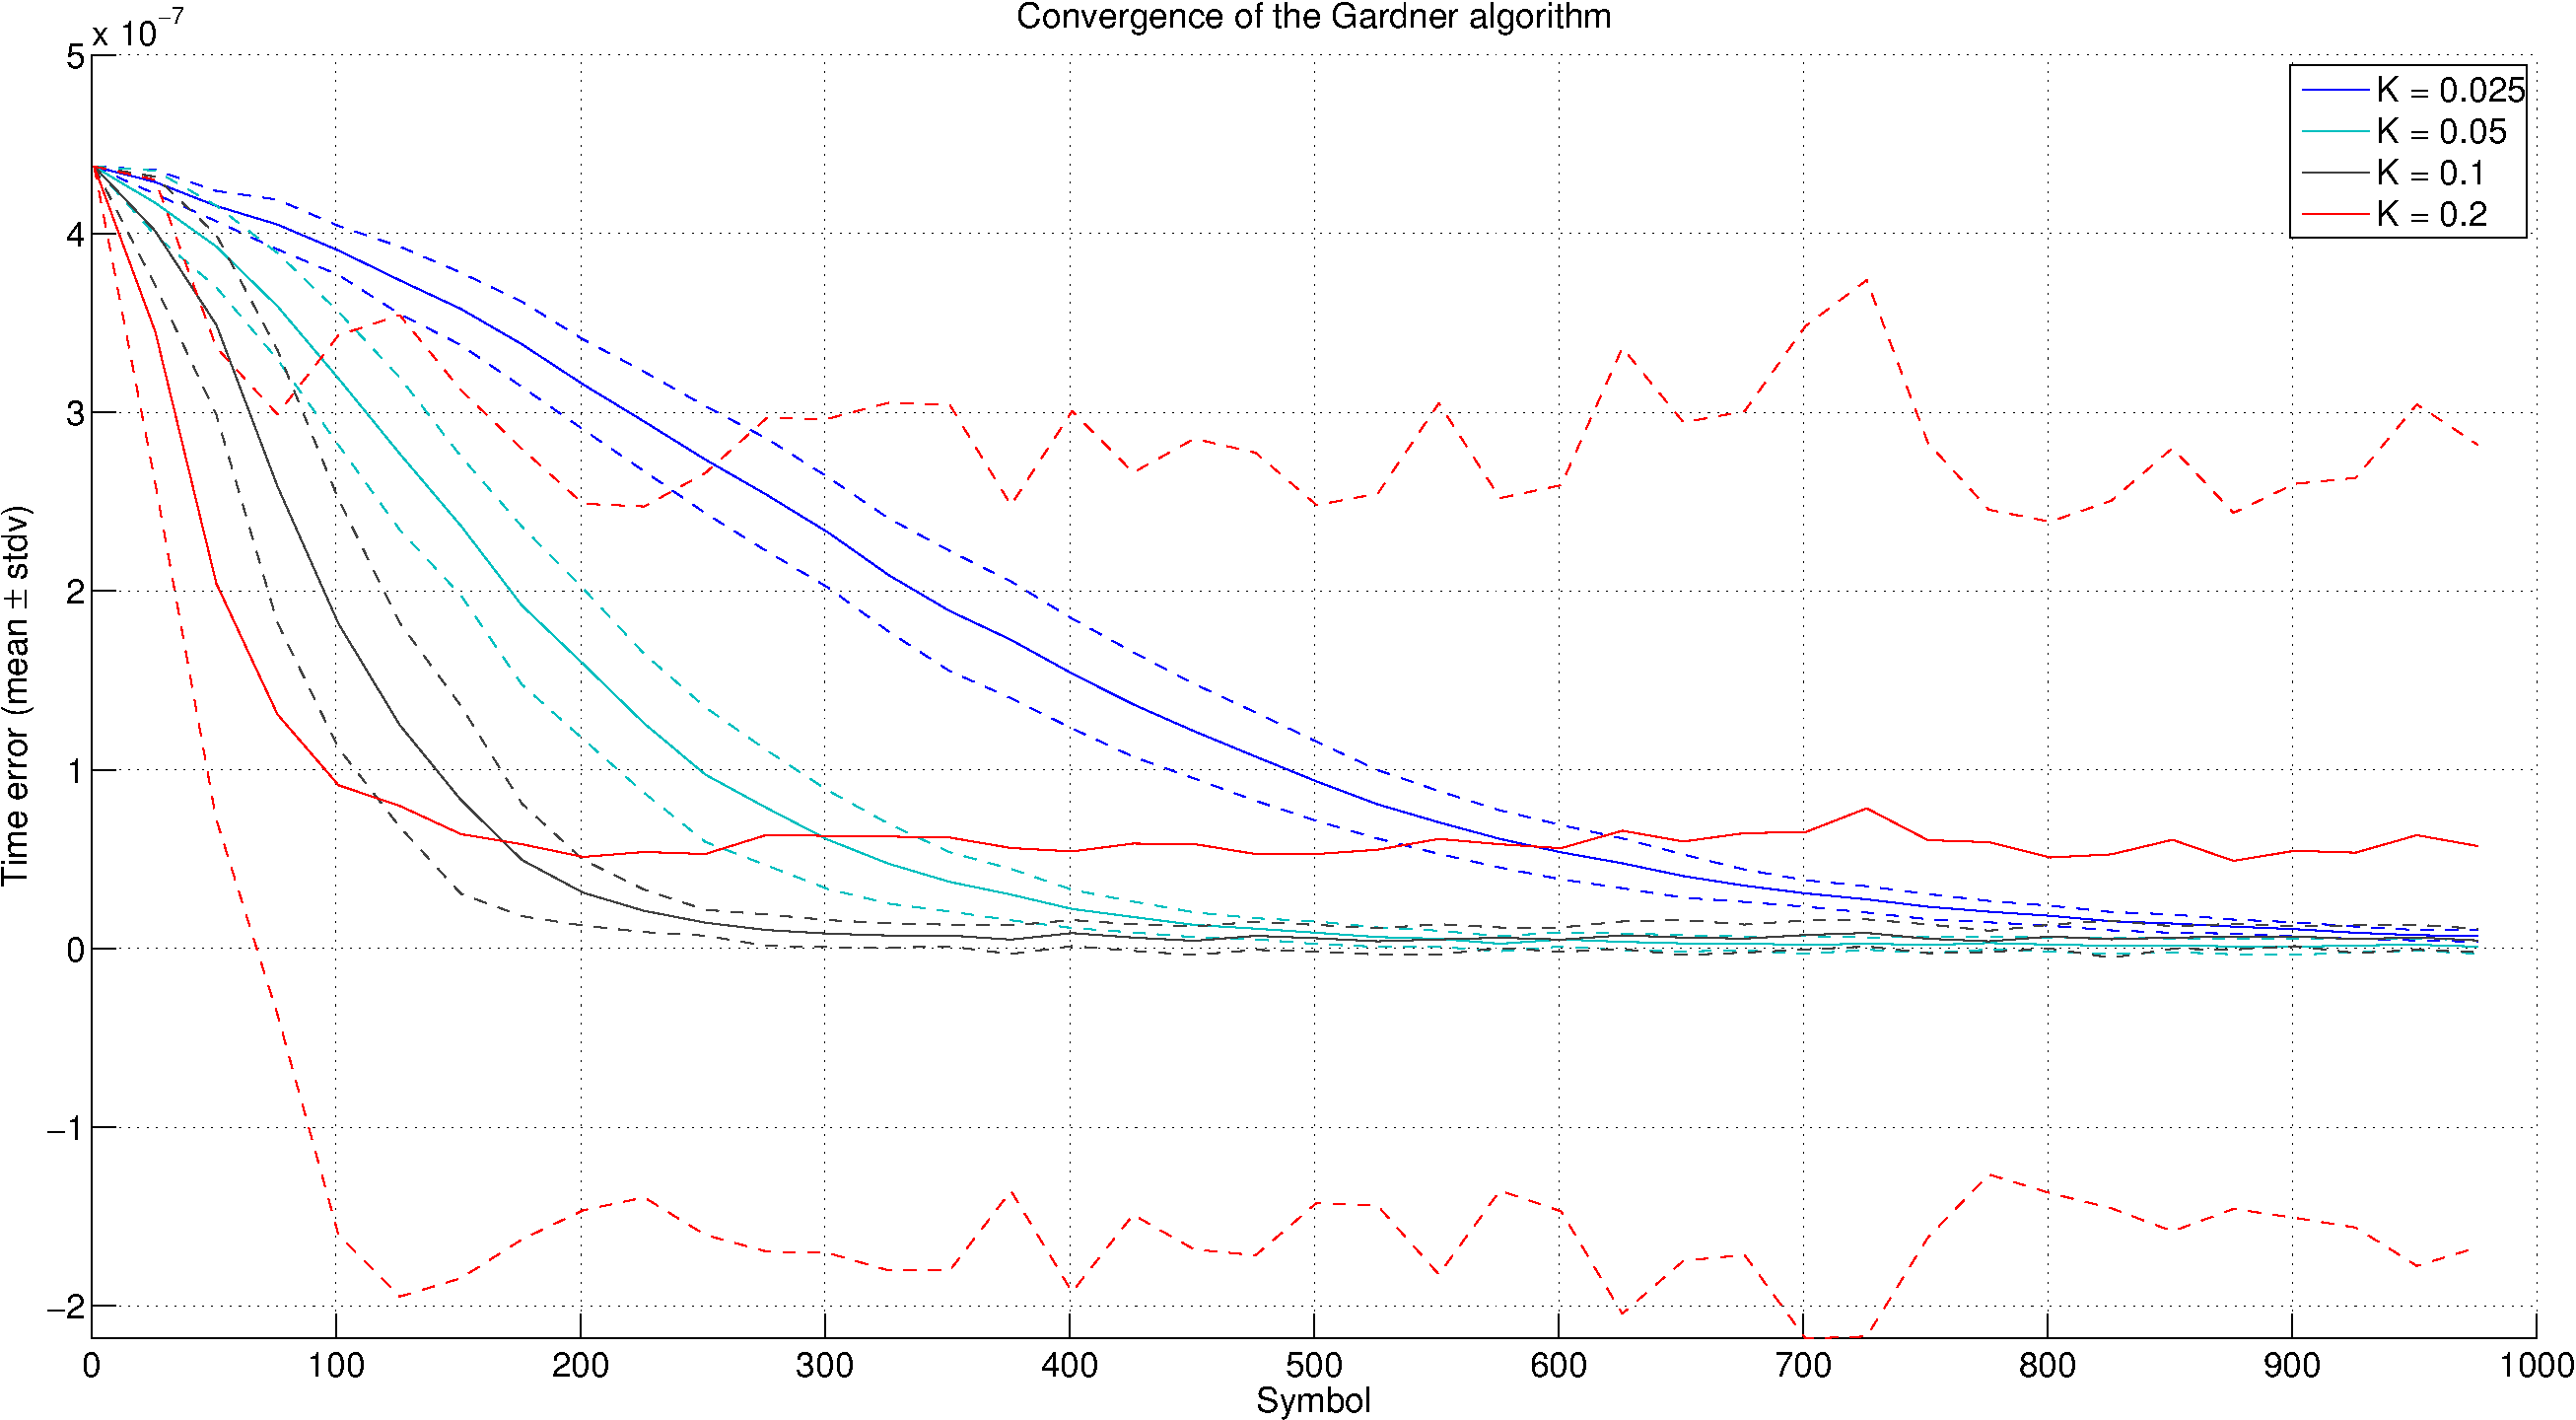
\includegraphics[width=\textwidth]{gardnerConverge.pdf}
    \caption[Convergence of the algorithm as a function of $\kappa$.]{Convergence of the algorithm as a function of $\kappa$. $\frac{E_b}{N_0} = \SI{10}{\decibel}$.\label{fig:gConvK}}
\end{figure}
As predicted by the theory, the algorithm converges faster for higher values of $\kappa$, but at the expense of accuracy and stability.

The resistance of the algorithm to CFO is shown in figure~\ref{fig:gConvCFO}.
\begin{figure}[htbp]
    \centering
    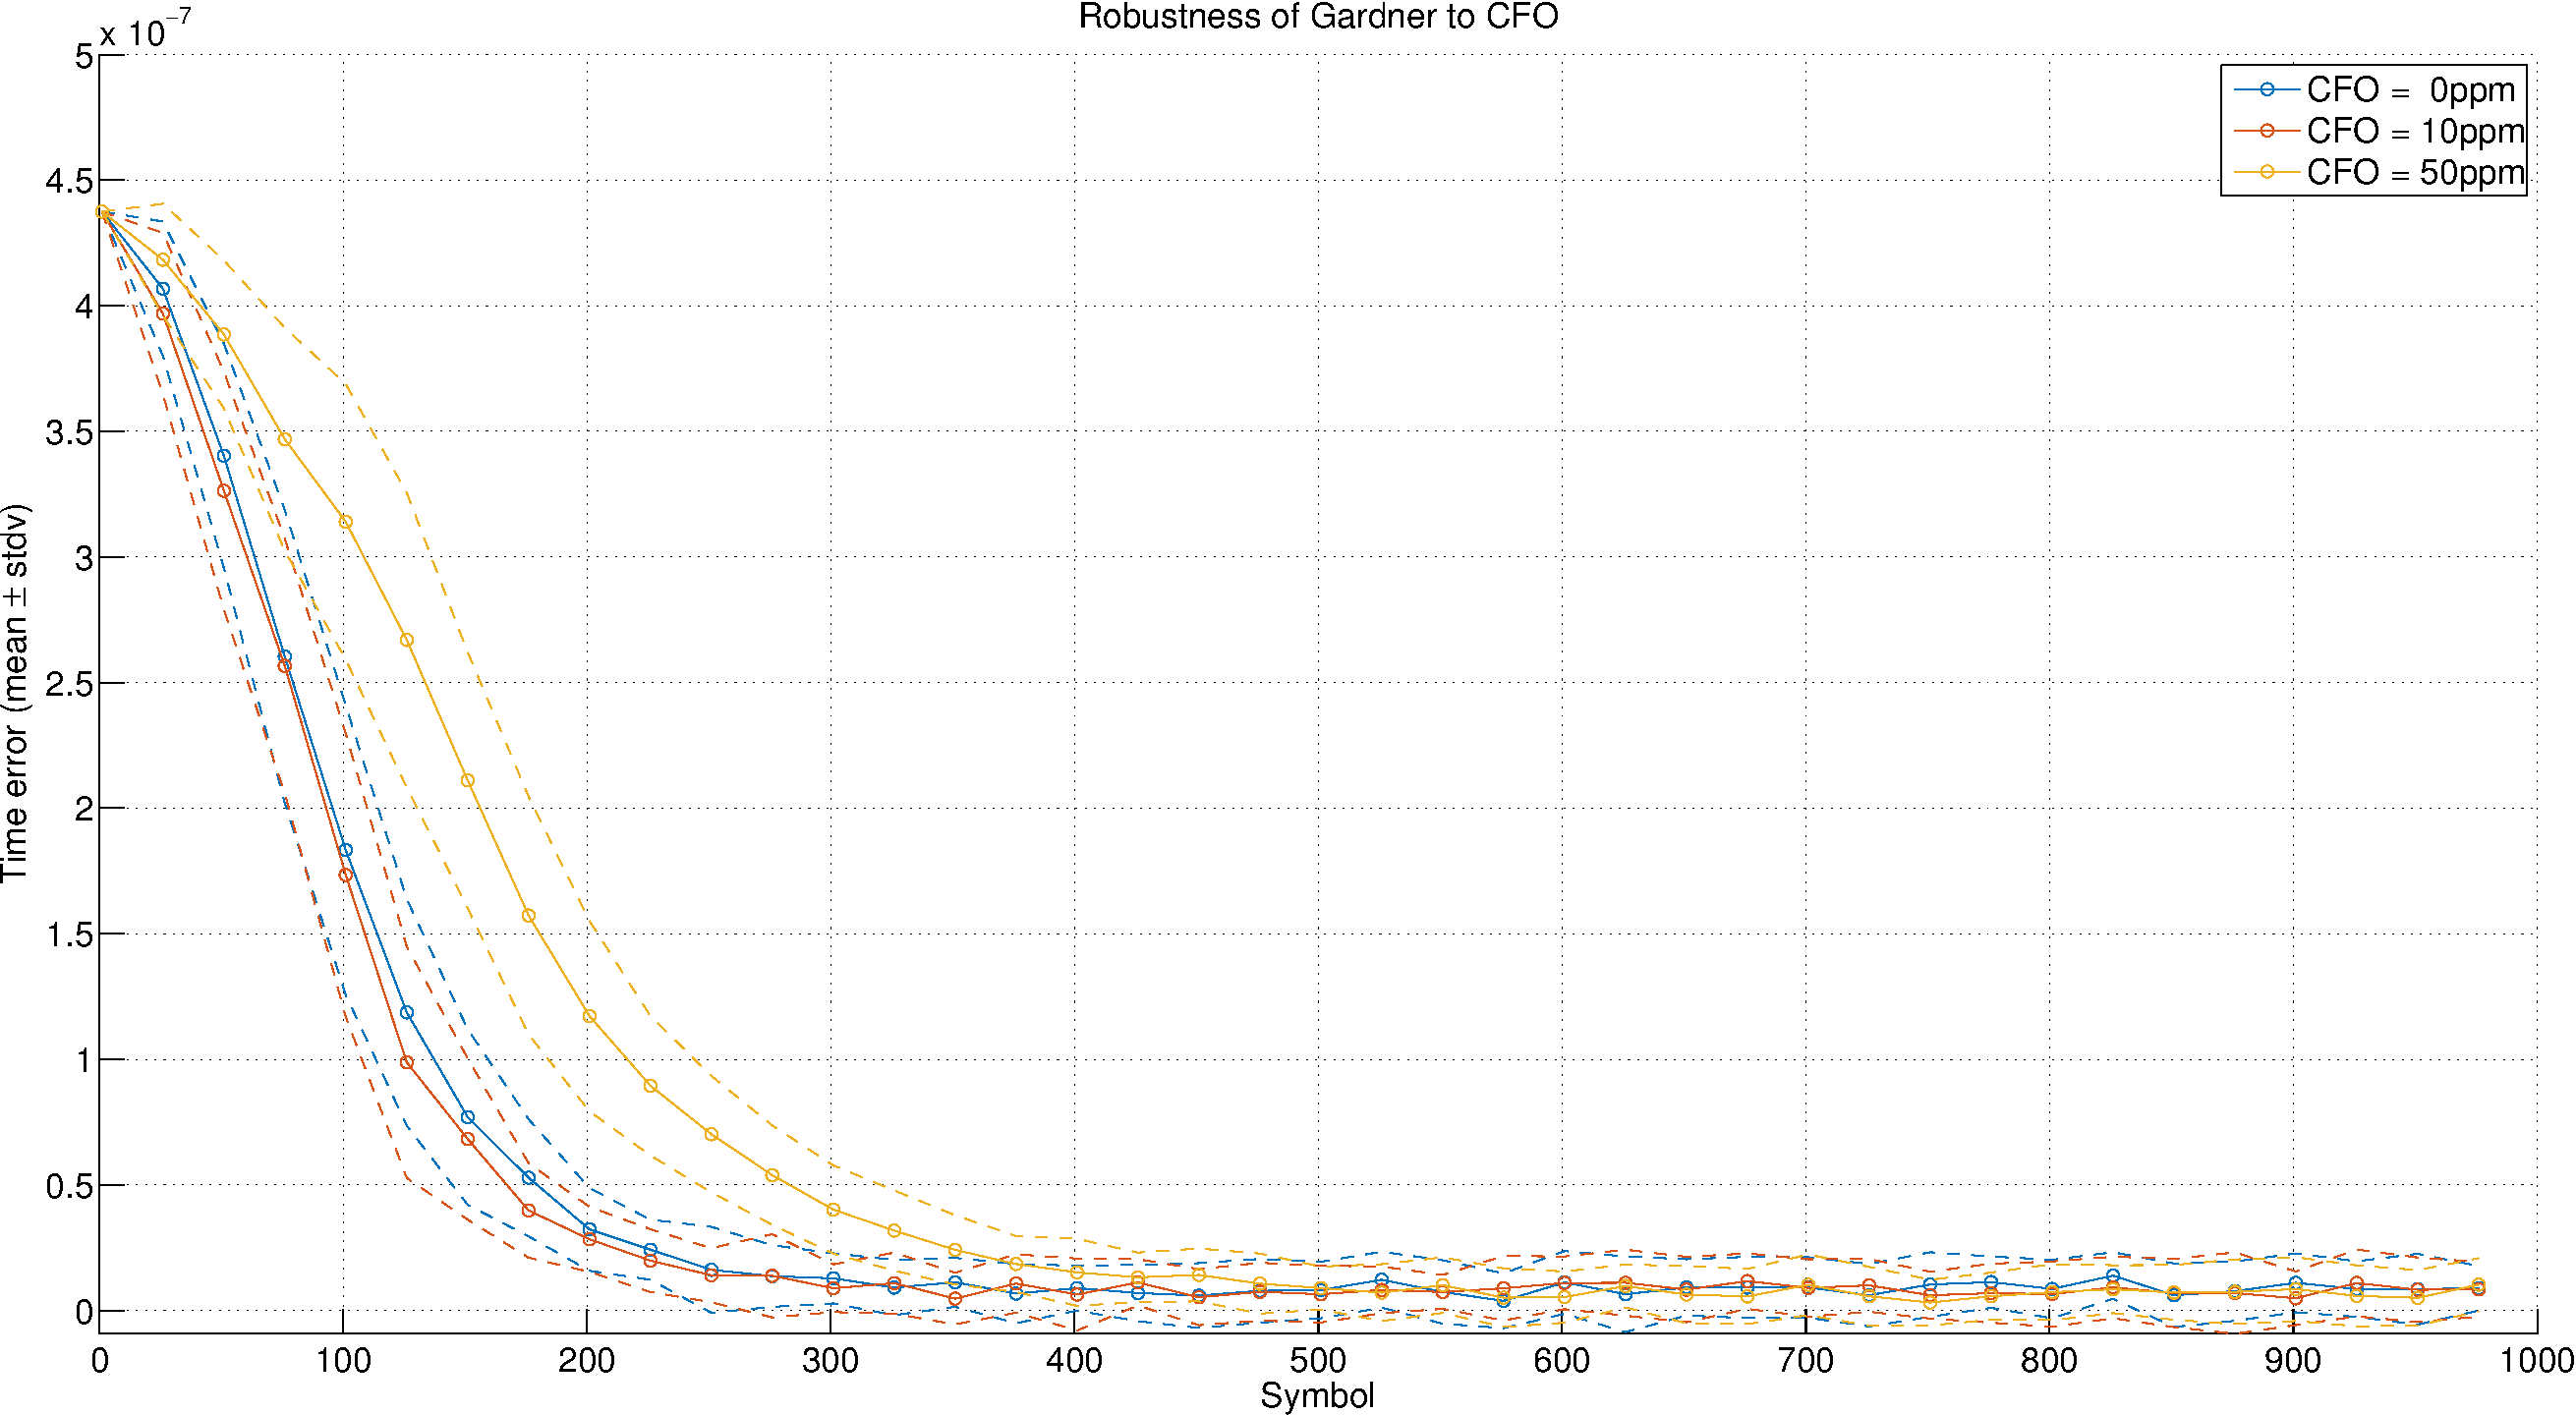
\includegraphics[width = \textwidth]{gardnerCFO2.pdf}
    \caption{Convergence of the algorithm as a function of the CFO.\label{fig:gConvCFO}}
\end{figure}
We see that for a standard specified CFO value of \SI{10}{\ppm}, the Gardner algorithm still converges satisfyingly.

\subsection{Time of Arrival and CFO Estimation Using Frame Acquisition}
In a practical application, the receiver doesn't know when the emitter will start to transmit a message.
In the case of a continuous stream, the receiver still has to resynchronize regularly because of the synchronization imperfections we discussed in the introduction to this section.
This is done by using differential cross-correlation to a pilot sequence which is repeatedly inserted in the stream of data blocks.
Using this cross correlator, it is possible to obtain an estimation of the time of arrival (ToA), meaning the position of the first bit of the frame in the incoming sequence, and of the CFO.
In addition to regularly reestimating the CFO and ToA which can slowly drift over time, the regularly spaced pilot sequences allow to refine the CFO estimation using frame interpolation.

The first output metric of the differential cross-correlator is shown in figure~\ref{fig:sumdk}
\begin{figure}
  \centering
  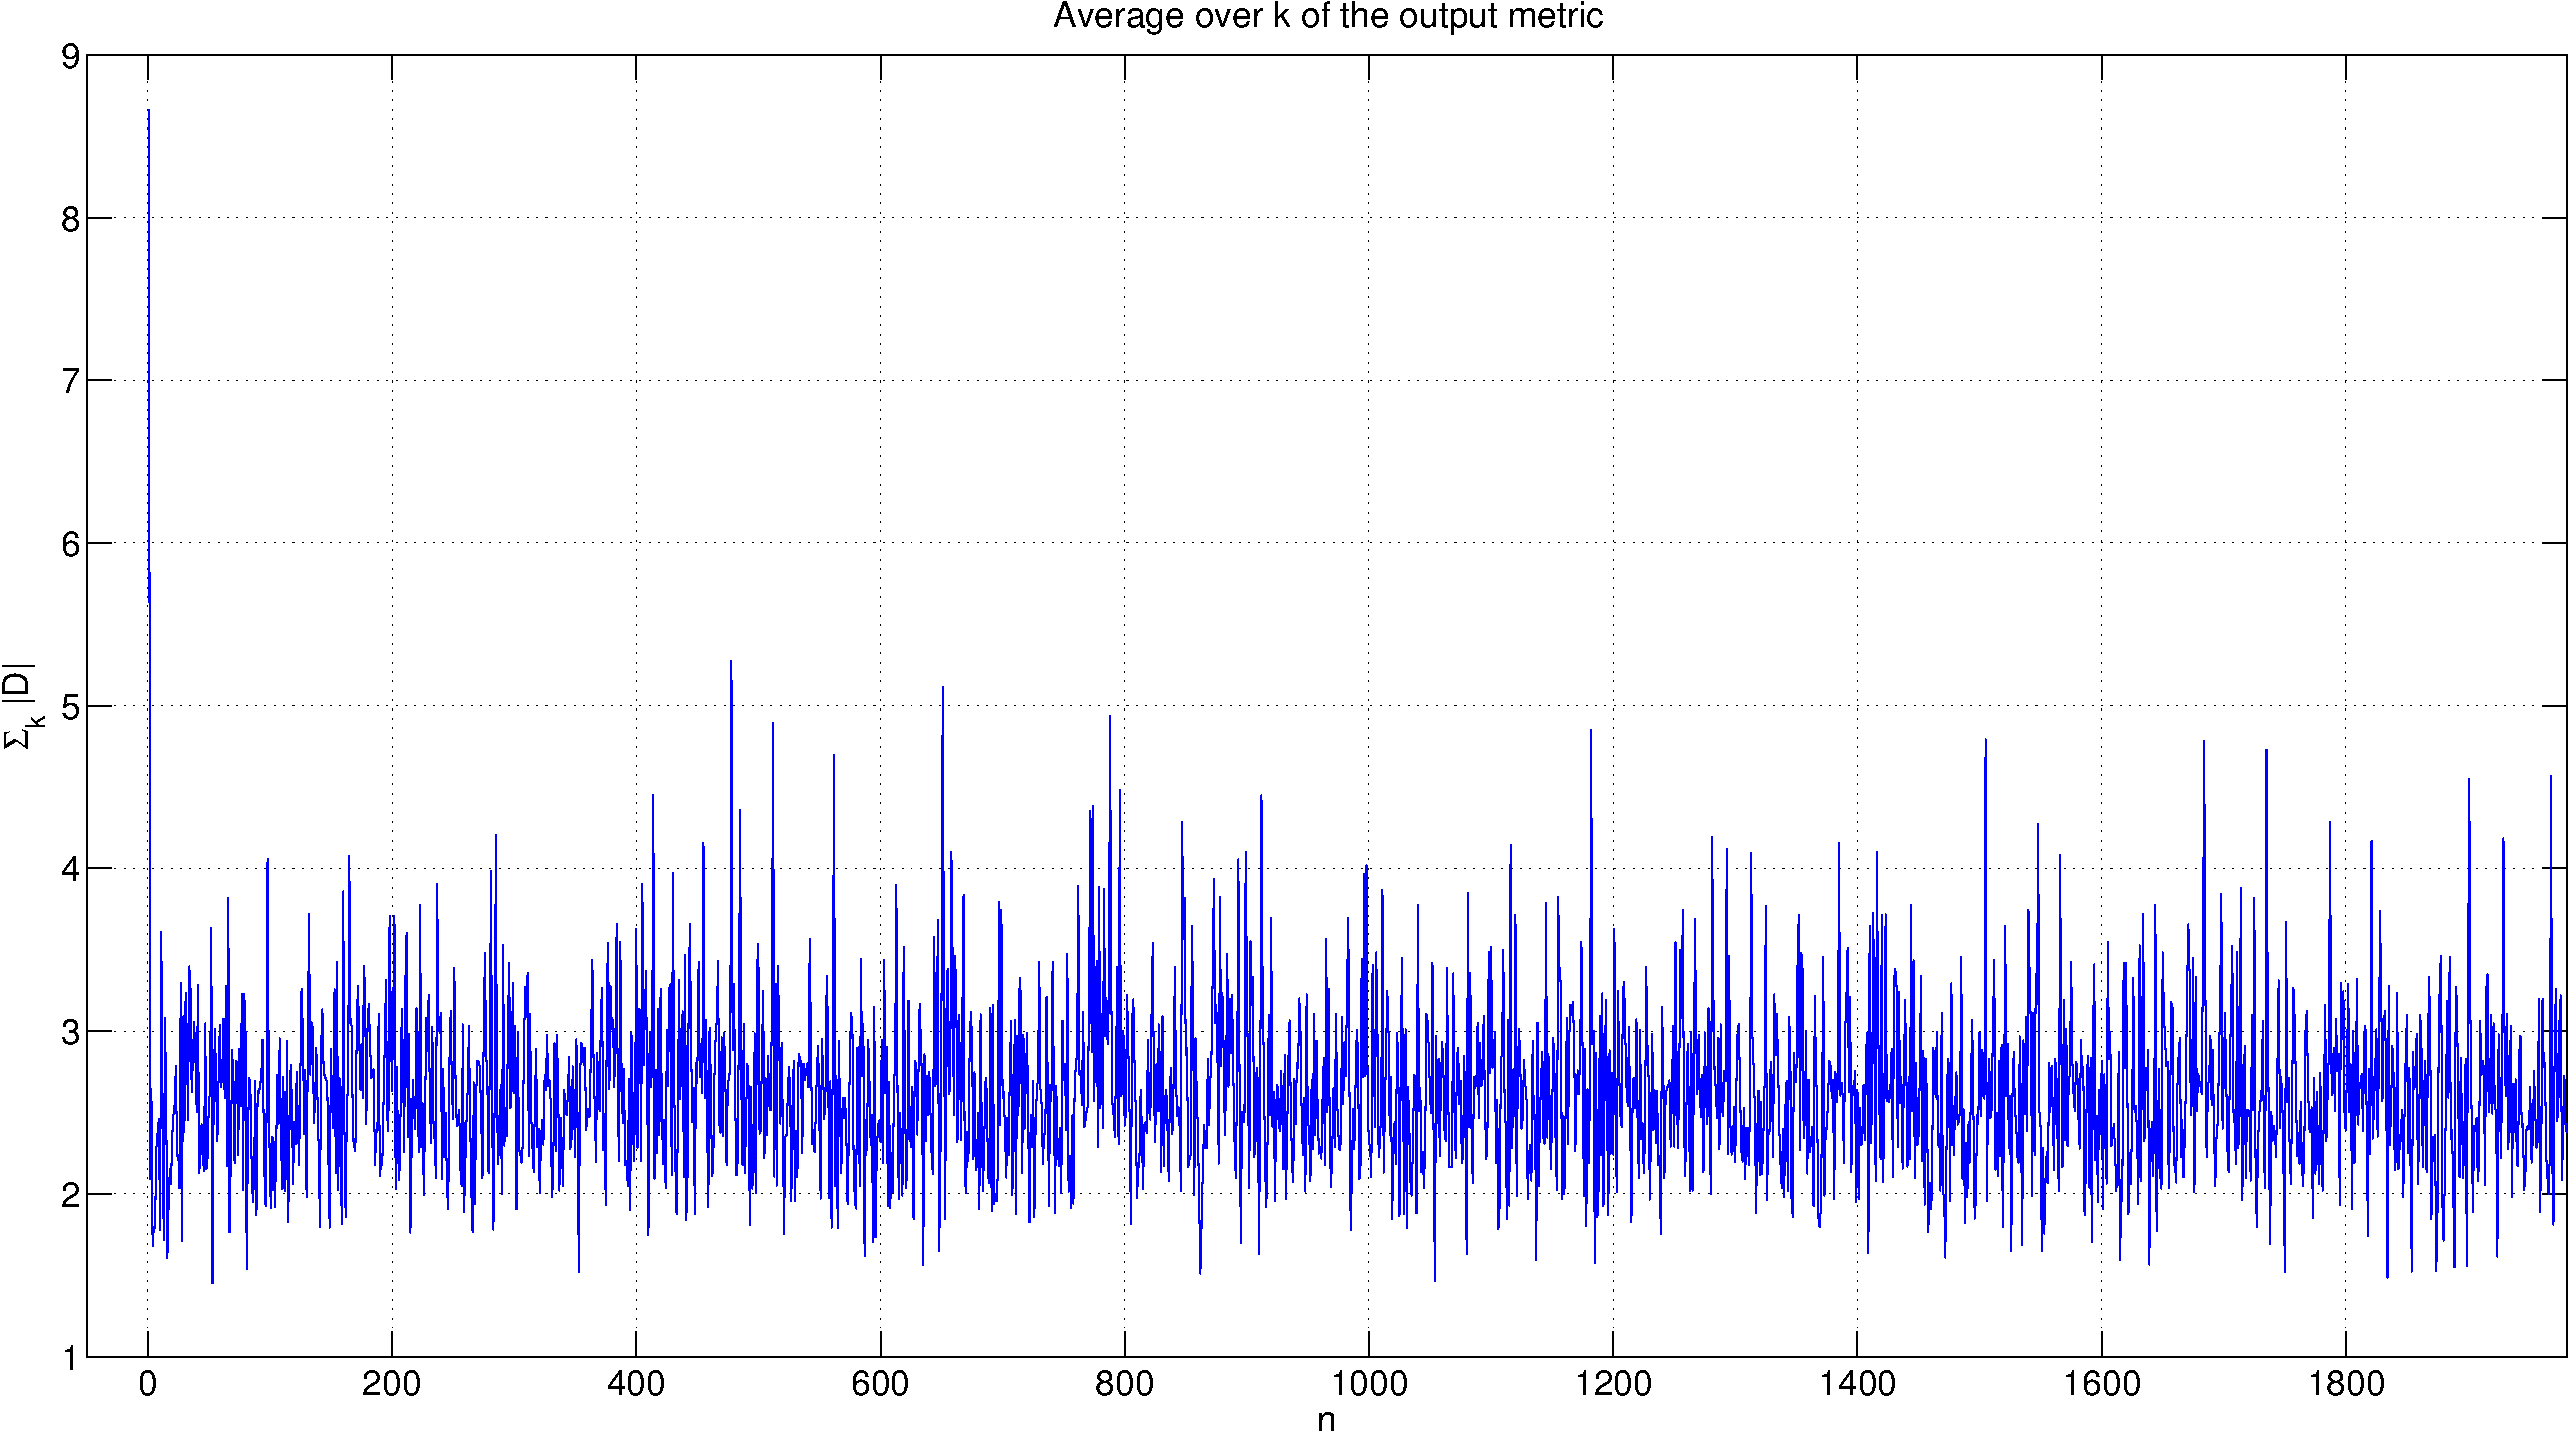
\includegraphics[width=\textwidth]{sumdk.pdf}
  \caption{ToA output metric.\label{fig:sumdk}}
\end{figure}
in order to illustrate the maximization over $n$ of $\sum_{k=1}^K |D_k[n]|$, for $N=40$ and $K = 8$. As expected, the output metric significantly at $n = 1$, which in this particular case is the true time of arrival.

Figure~\ref{fig:frametoa}
\begin{figure}
  \centering
  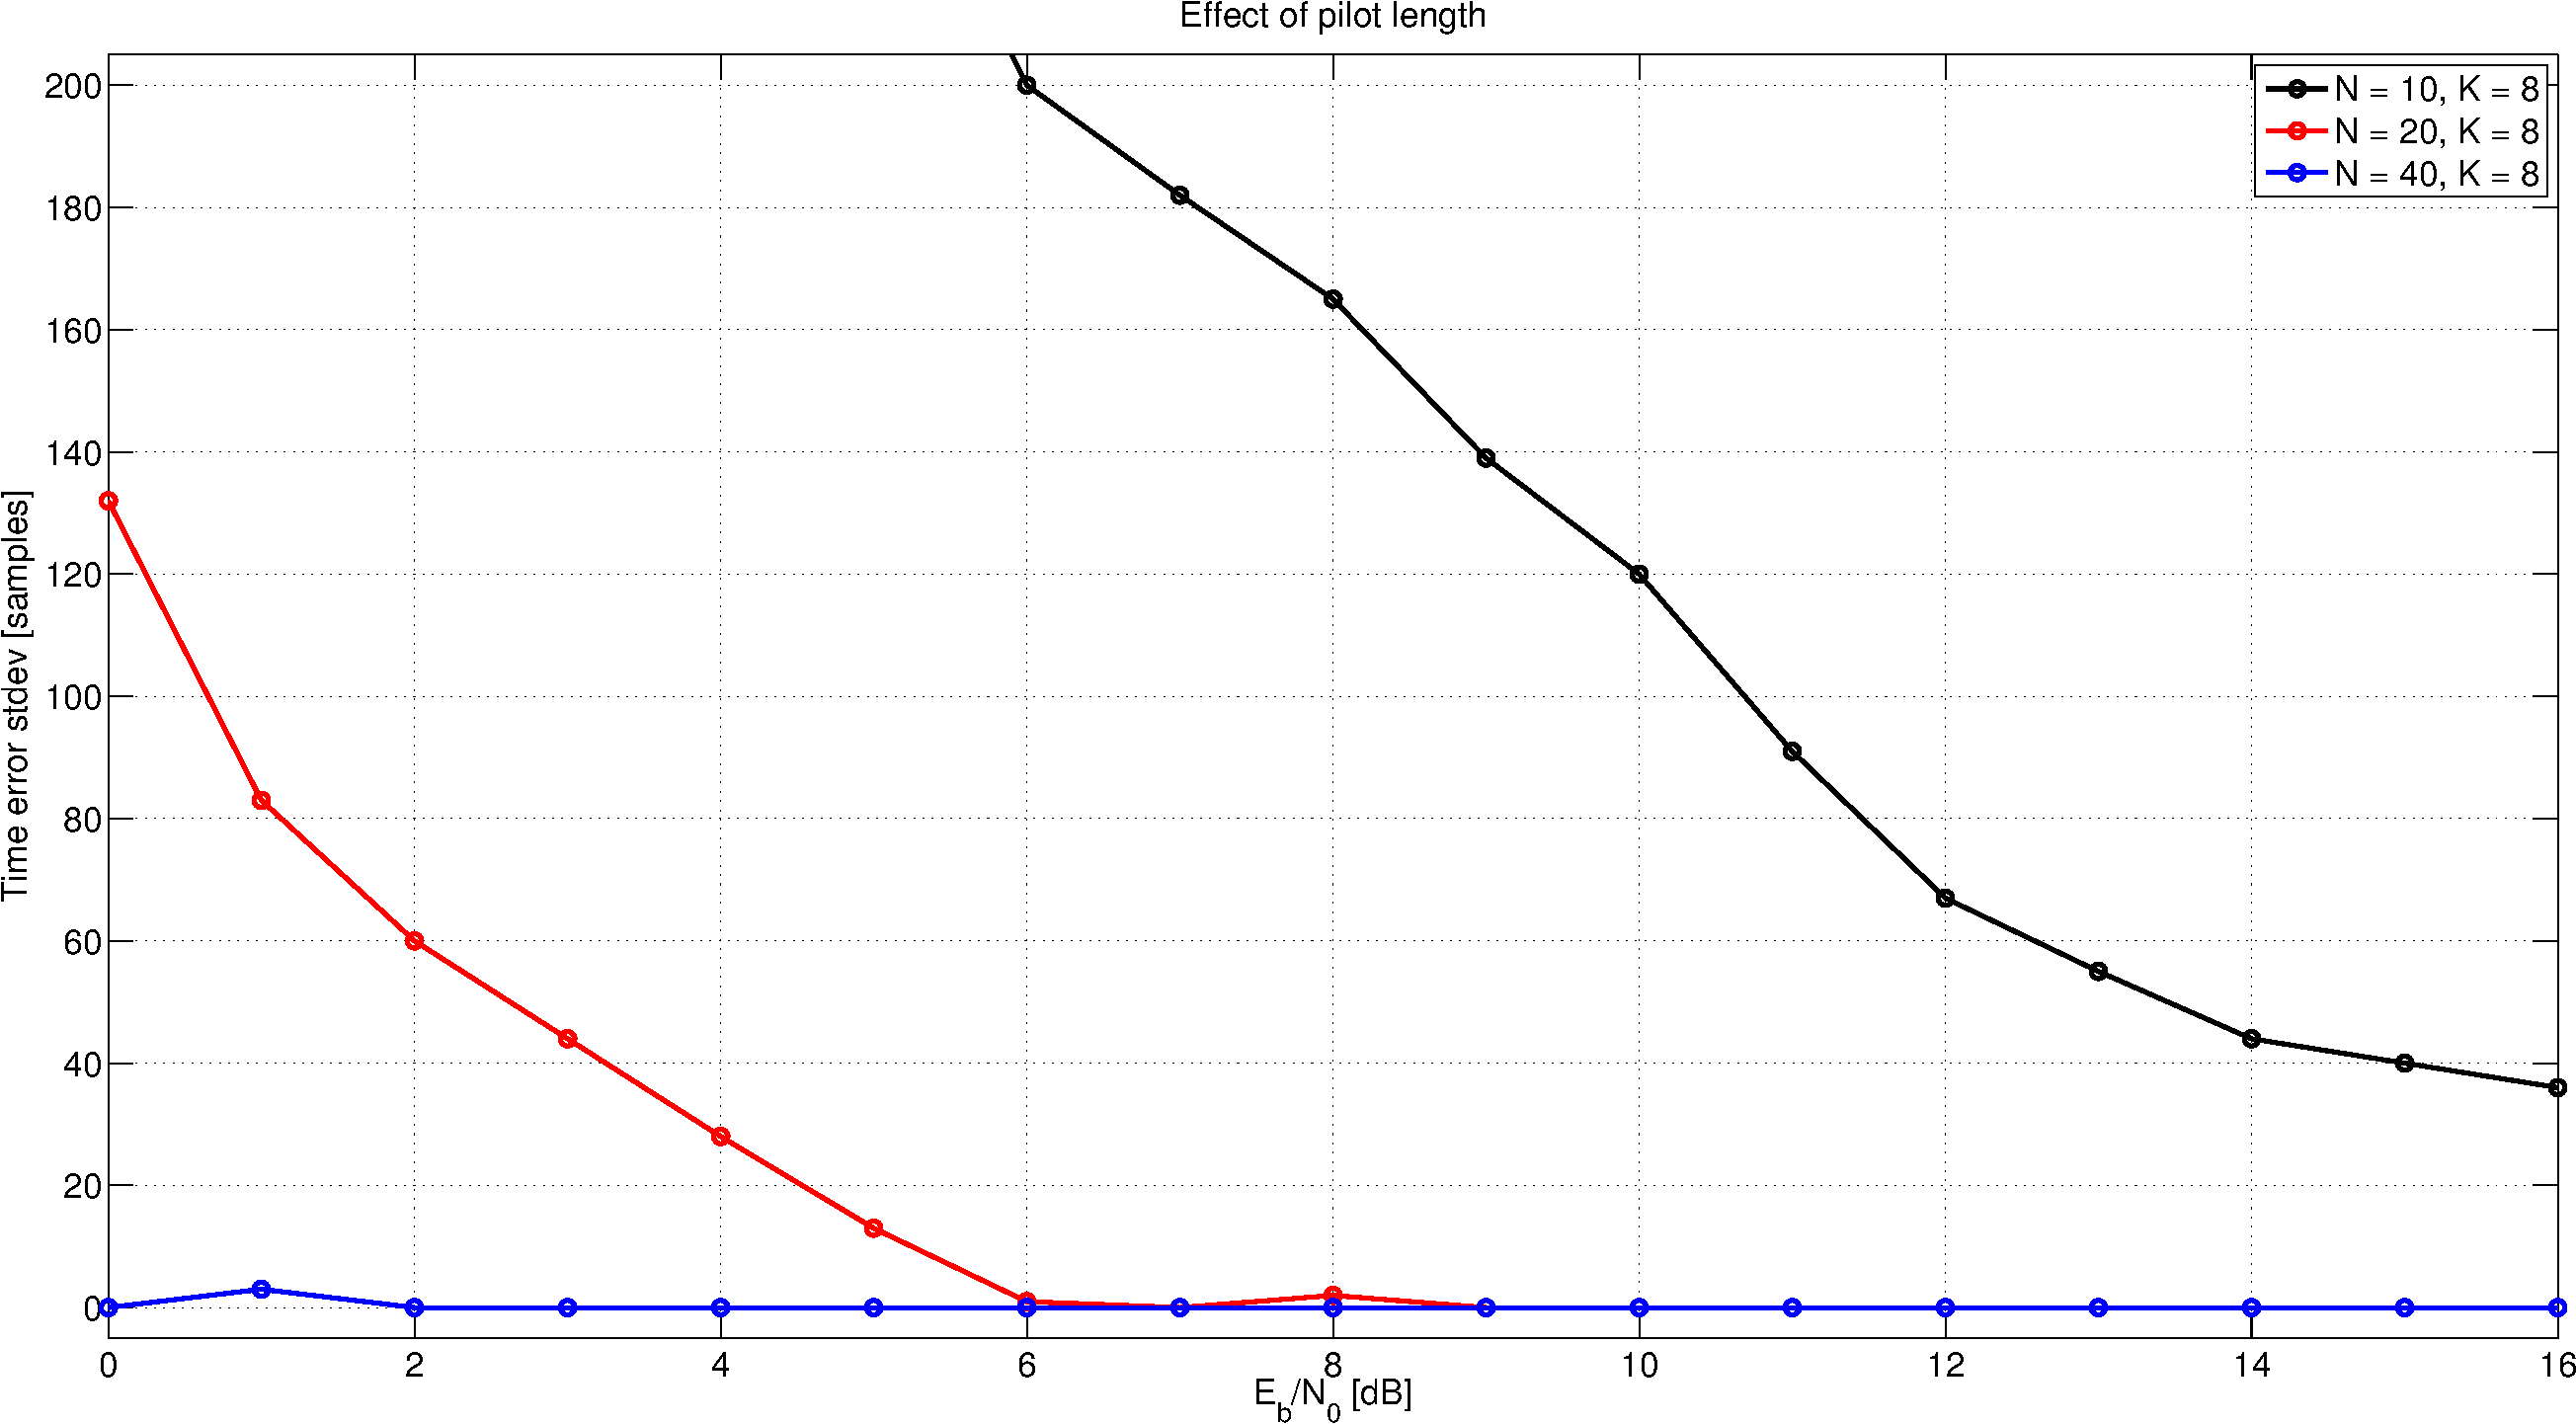
\includegraphics[width=\textwidth]{frametoan.pdf}
  \\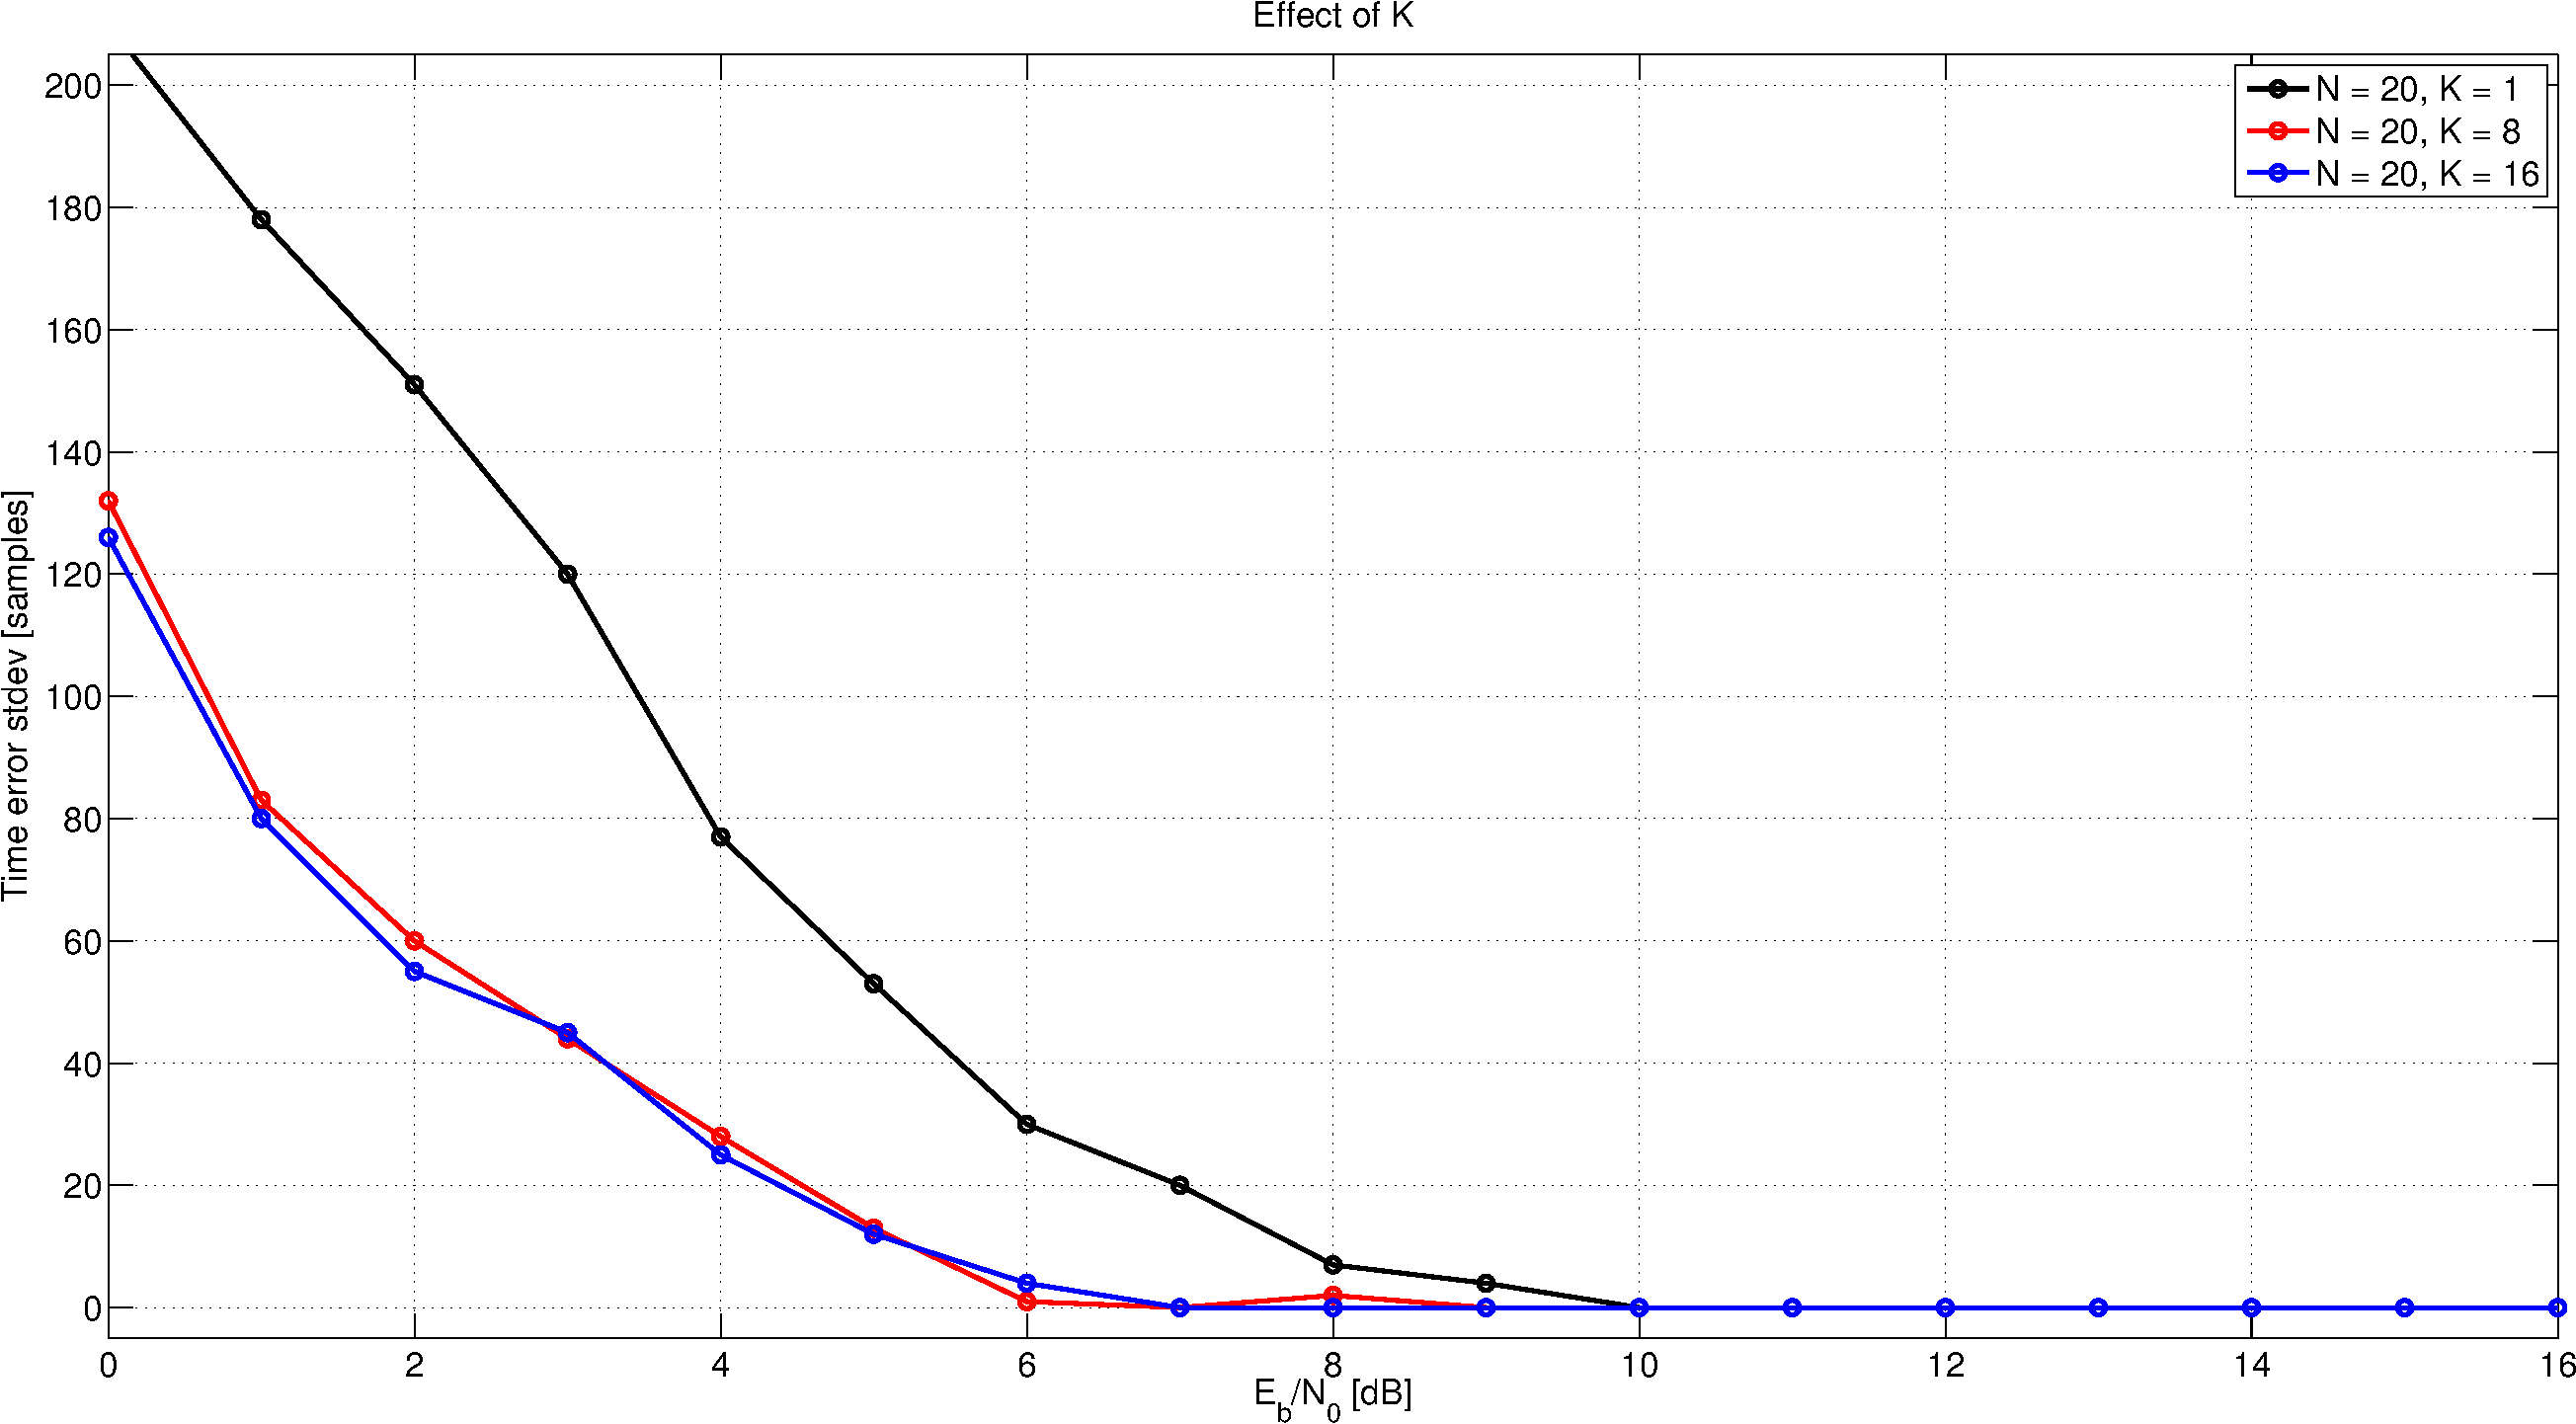
\includegraphics[width=\textwidth]{frametoak.pdf}
  \caption{Pilot ToA error as a function of N and K.\label{fig:frametoa}}
\end{figure}
shows the accuracy of the ToA estimation in function of N, K and the channel SNR for 4-QAM modulation.
Figure~\ref{fig:frametoacfo}
\begin{figure}
  \centering
  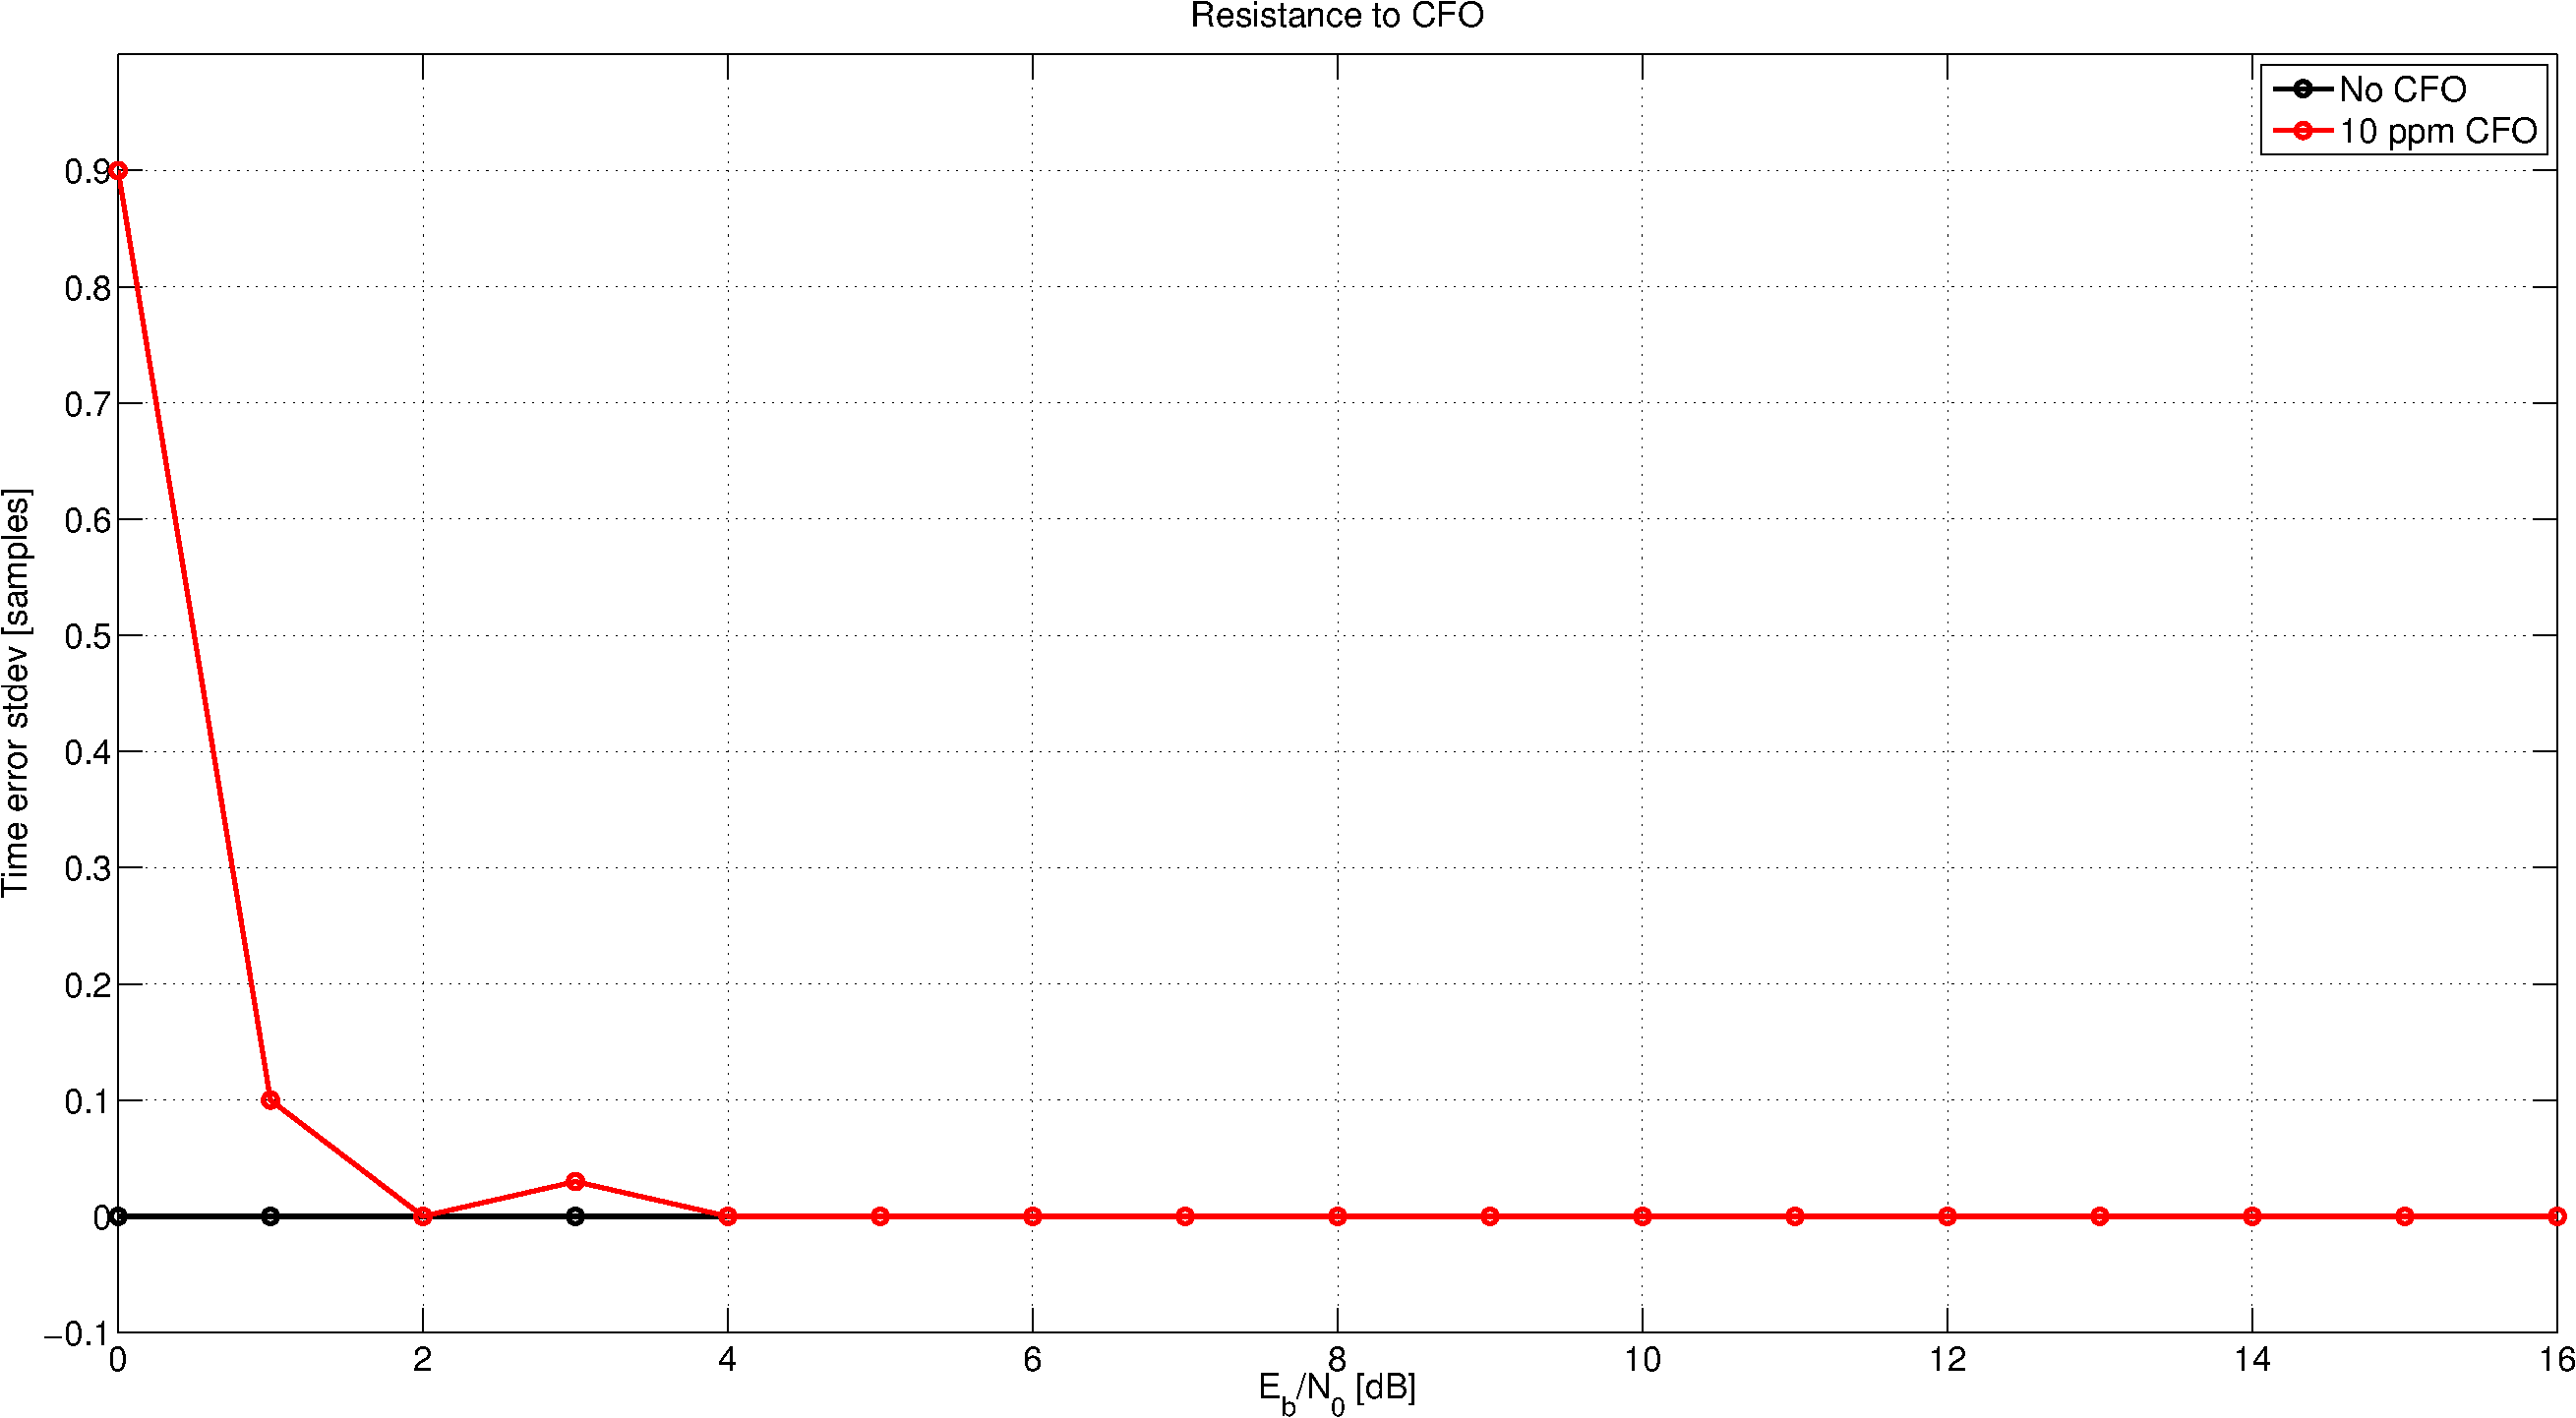
\includegraphics[width=\textwidth]{frametoacfo.pdf}
  \caption{Resistance of the ToA estimation to CFO.\label{fig:frametoacfo}}
\end{figure}
shows the resistance of the ToA estimation to CFO for 4-QAM modulation with $N = 40$ and $K=8$.

Figure~\ref{fig:framecfo}
\begin{figure}
  \centering
  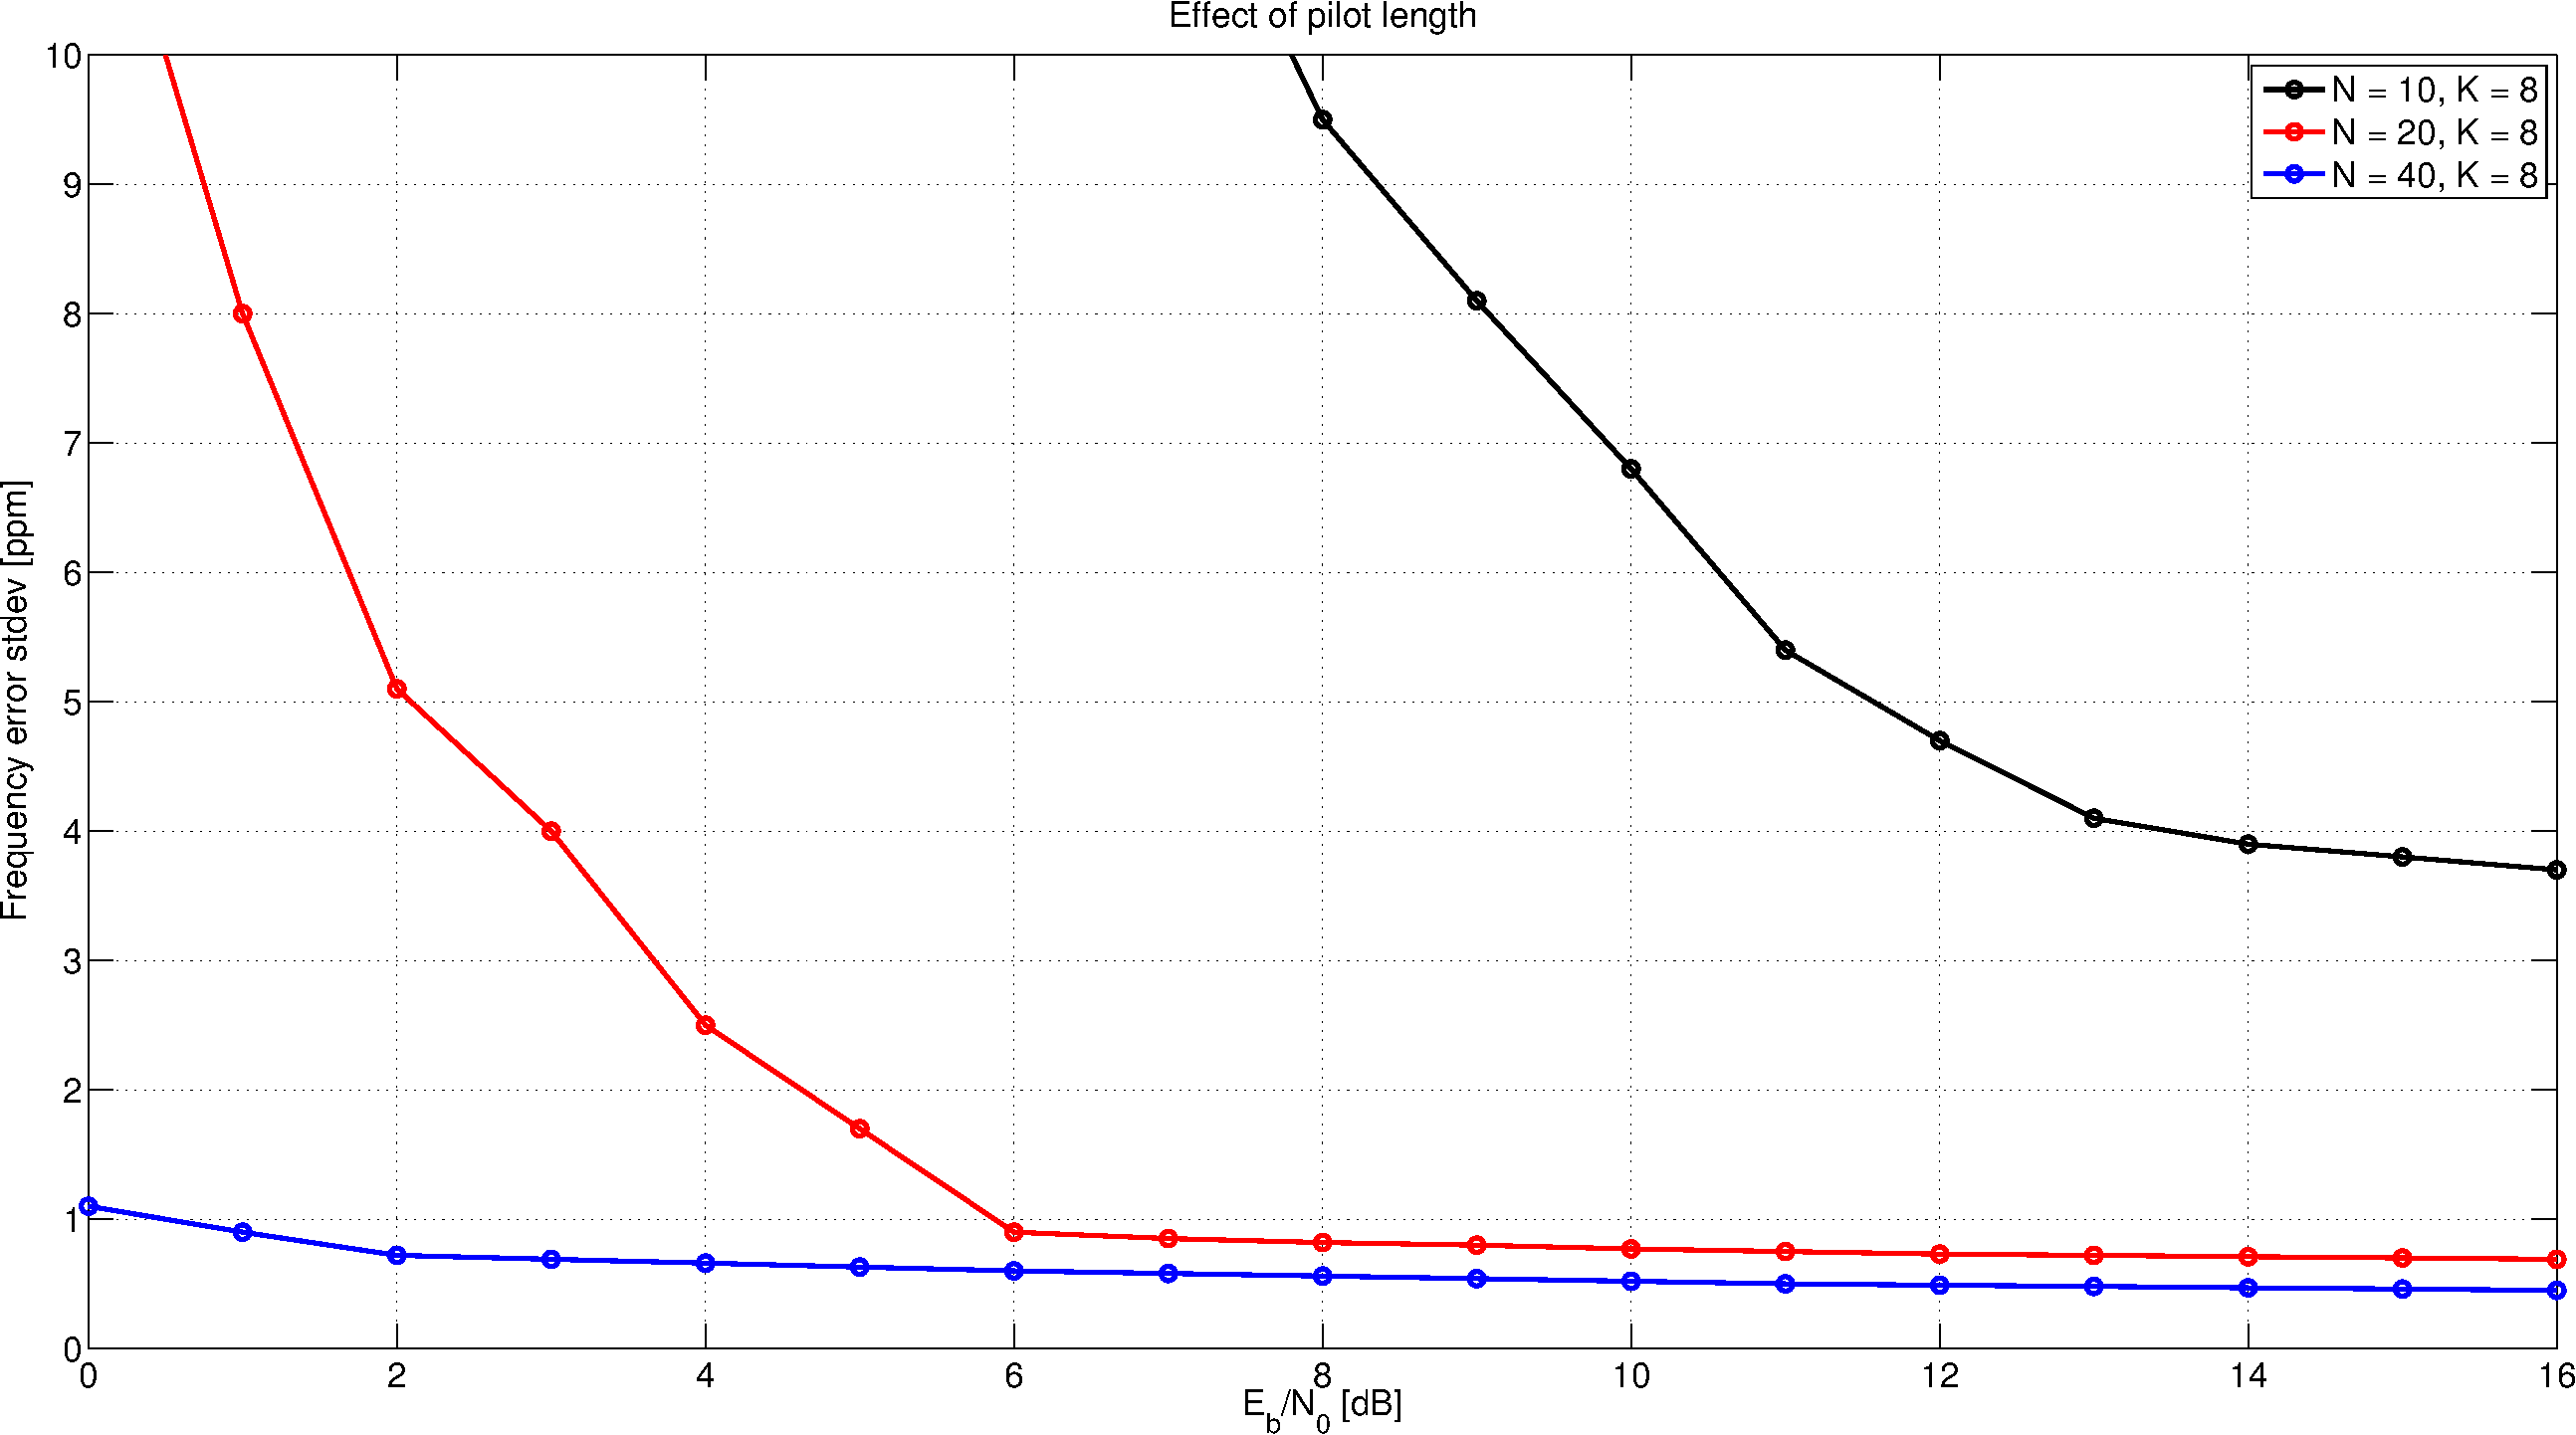
\includegraphics[width=\textwidth]{framecfon.pdf}
  \\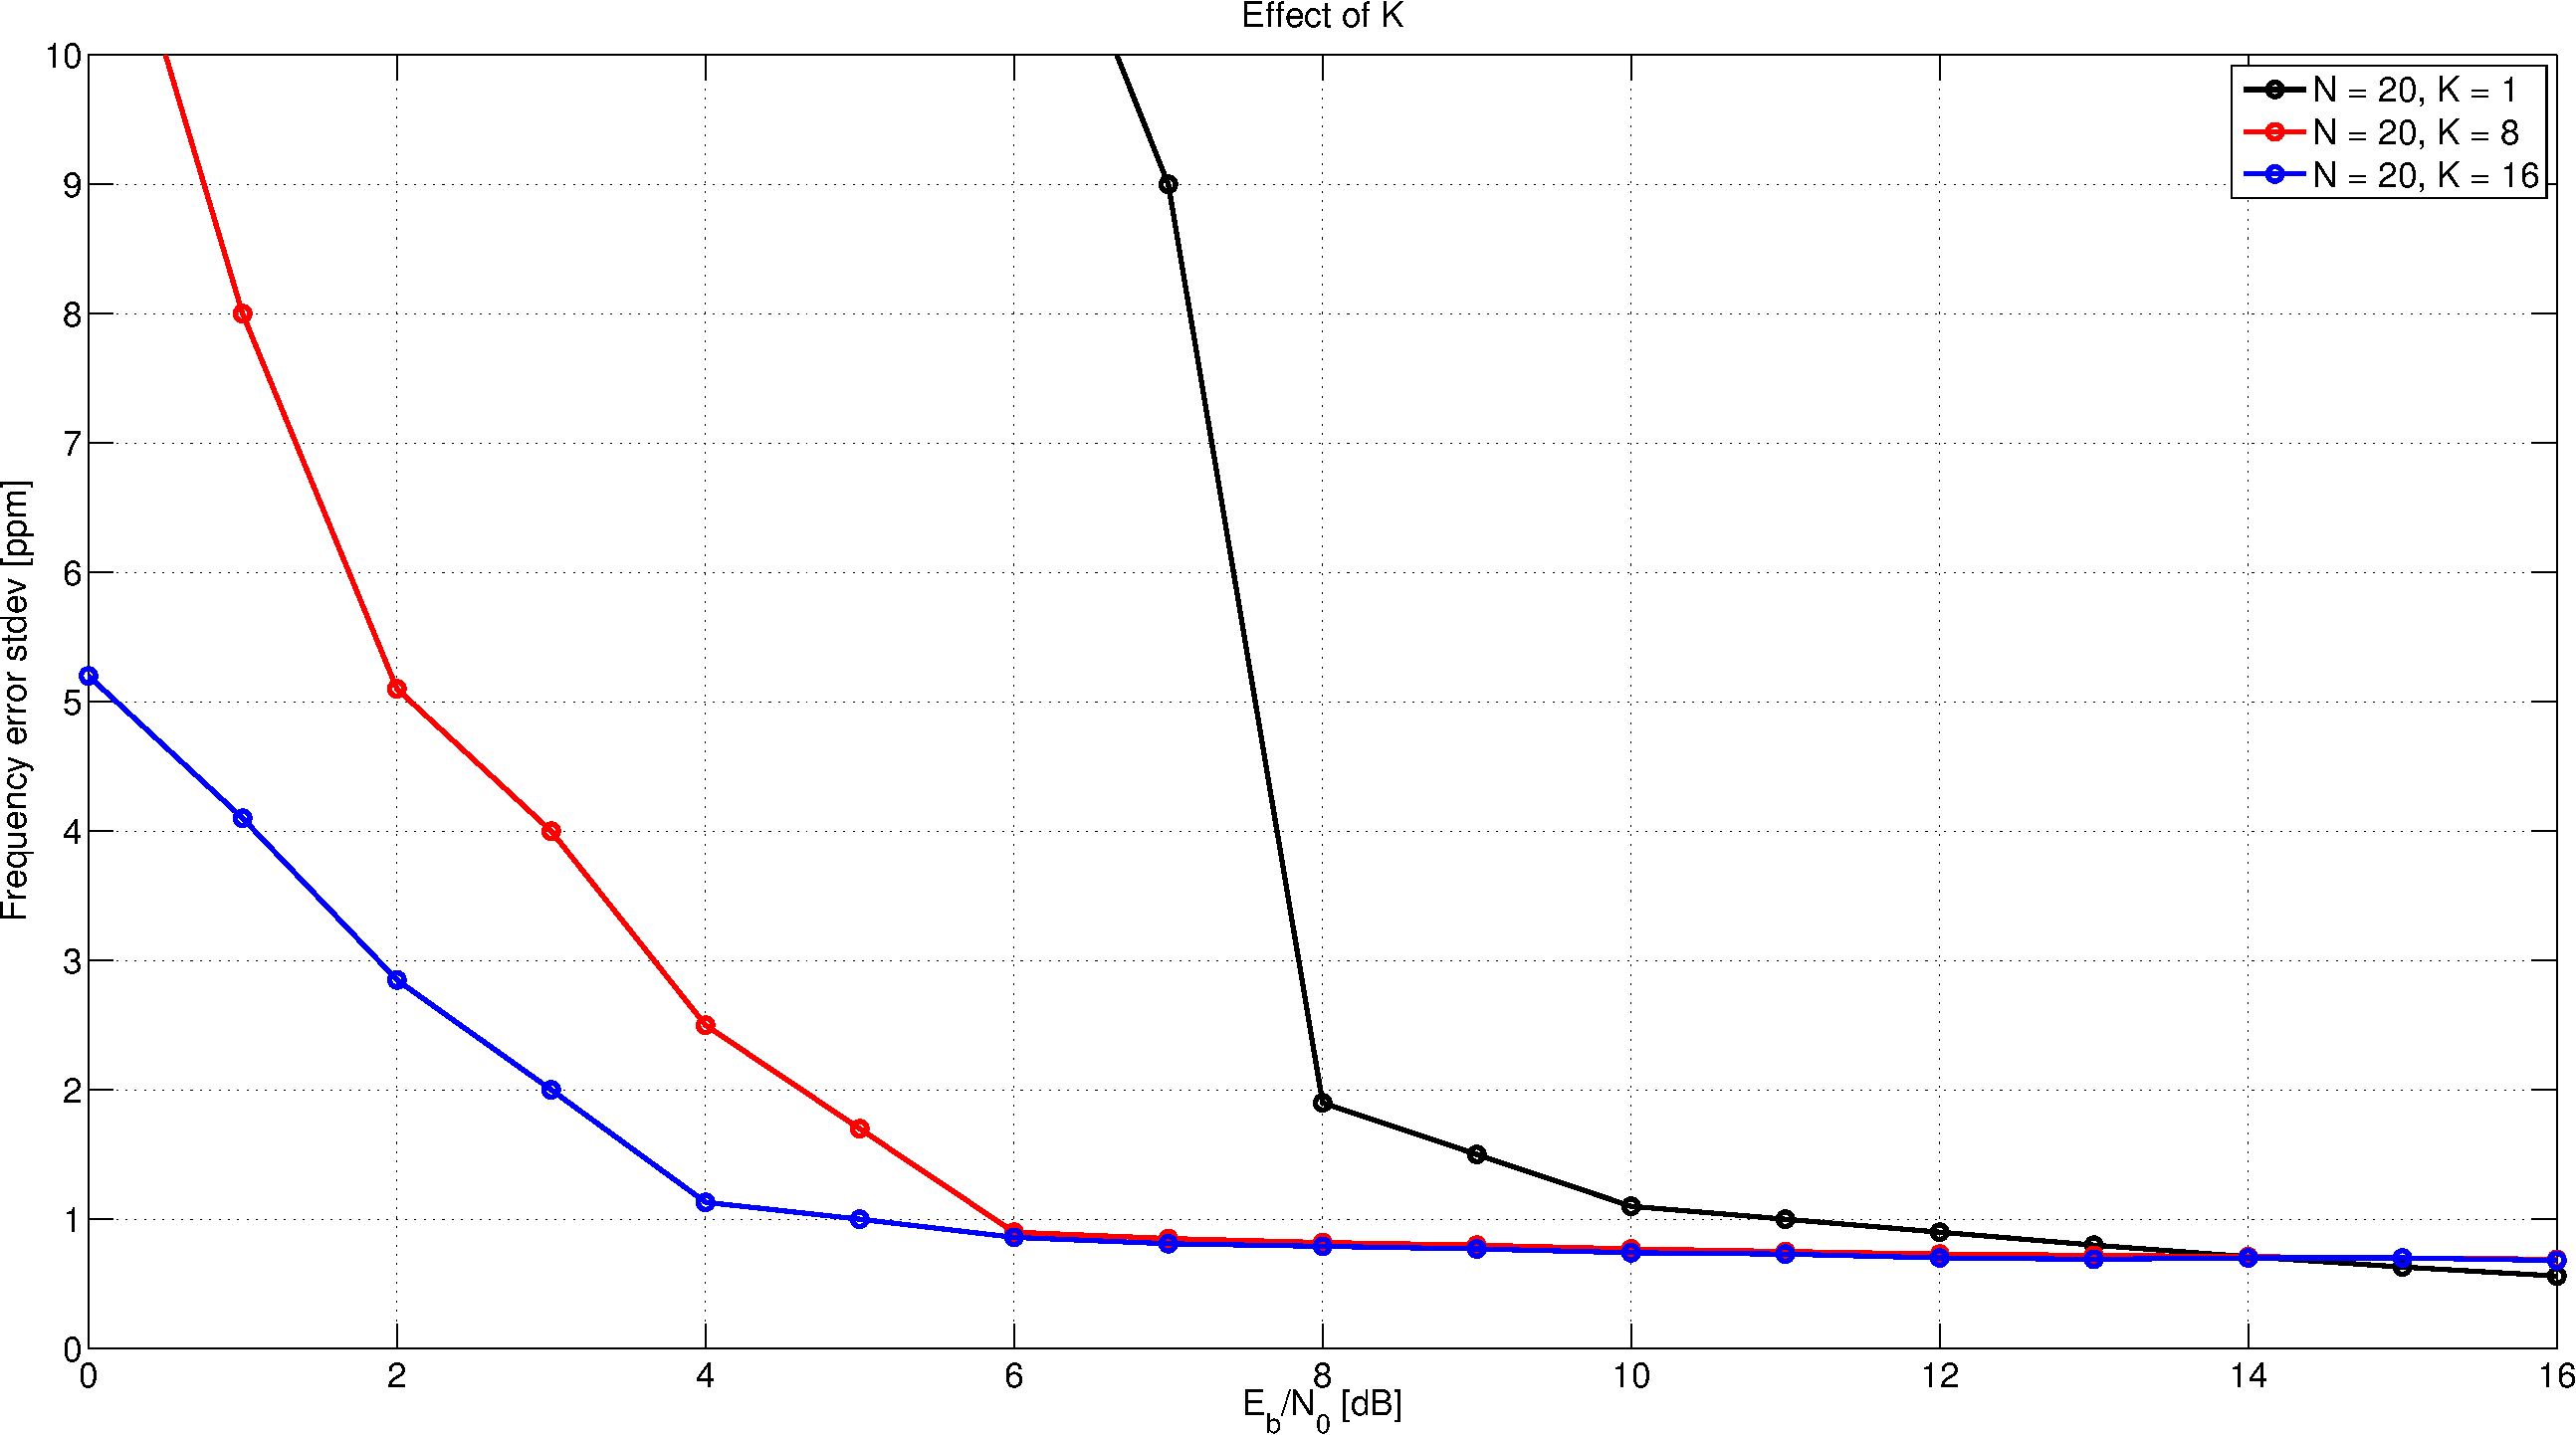
\includegraphics[width=\textwidth]{framecfok.pdf}
  \caption{CFO error as a function of N and K.\label{fig:framecfo}}
\end{figure}
shows the accuracy of the CFO estimation as a function of N, K and the channel SNR for 4-QAM modulation.
Figure~\ref{fig:framecfocfo}
\begin{figure}
  \centering
  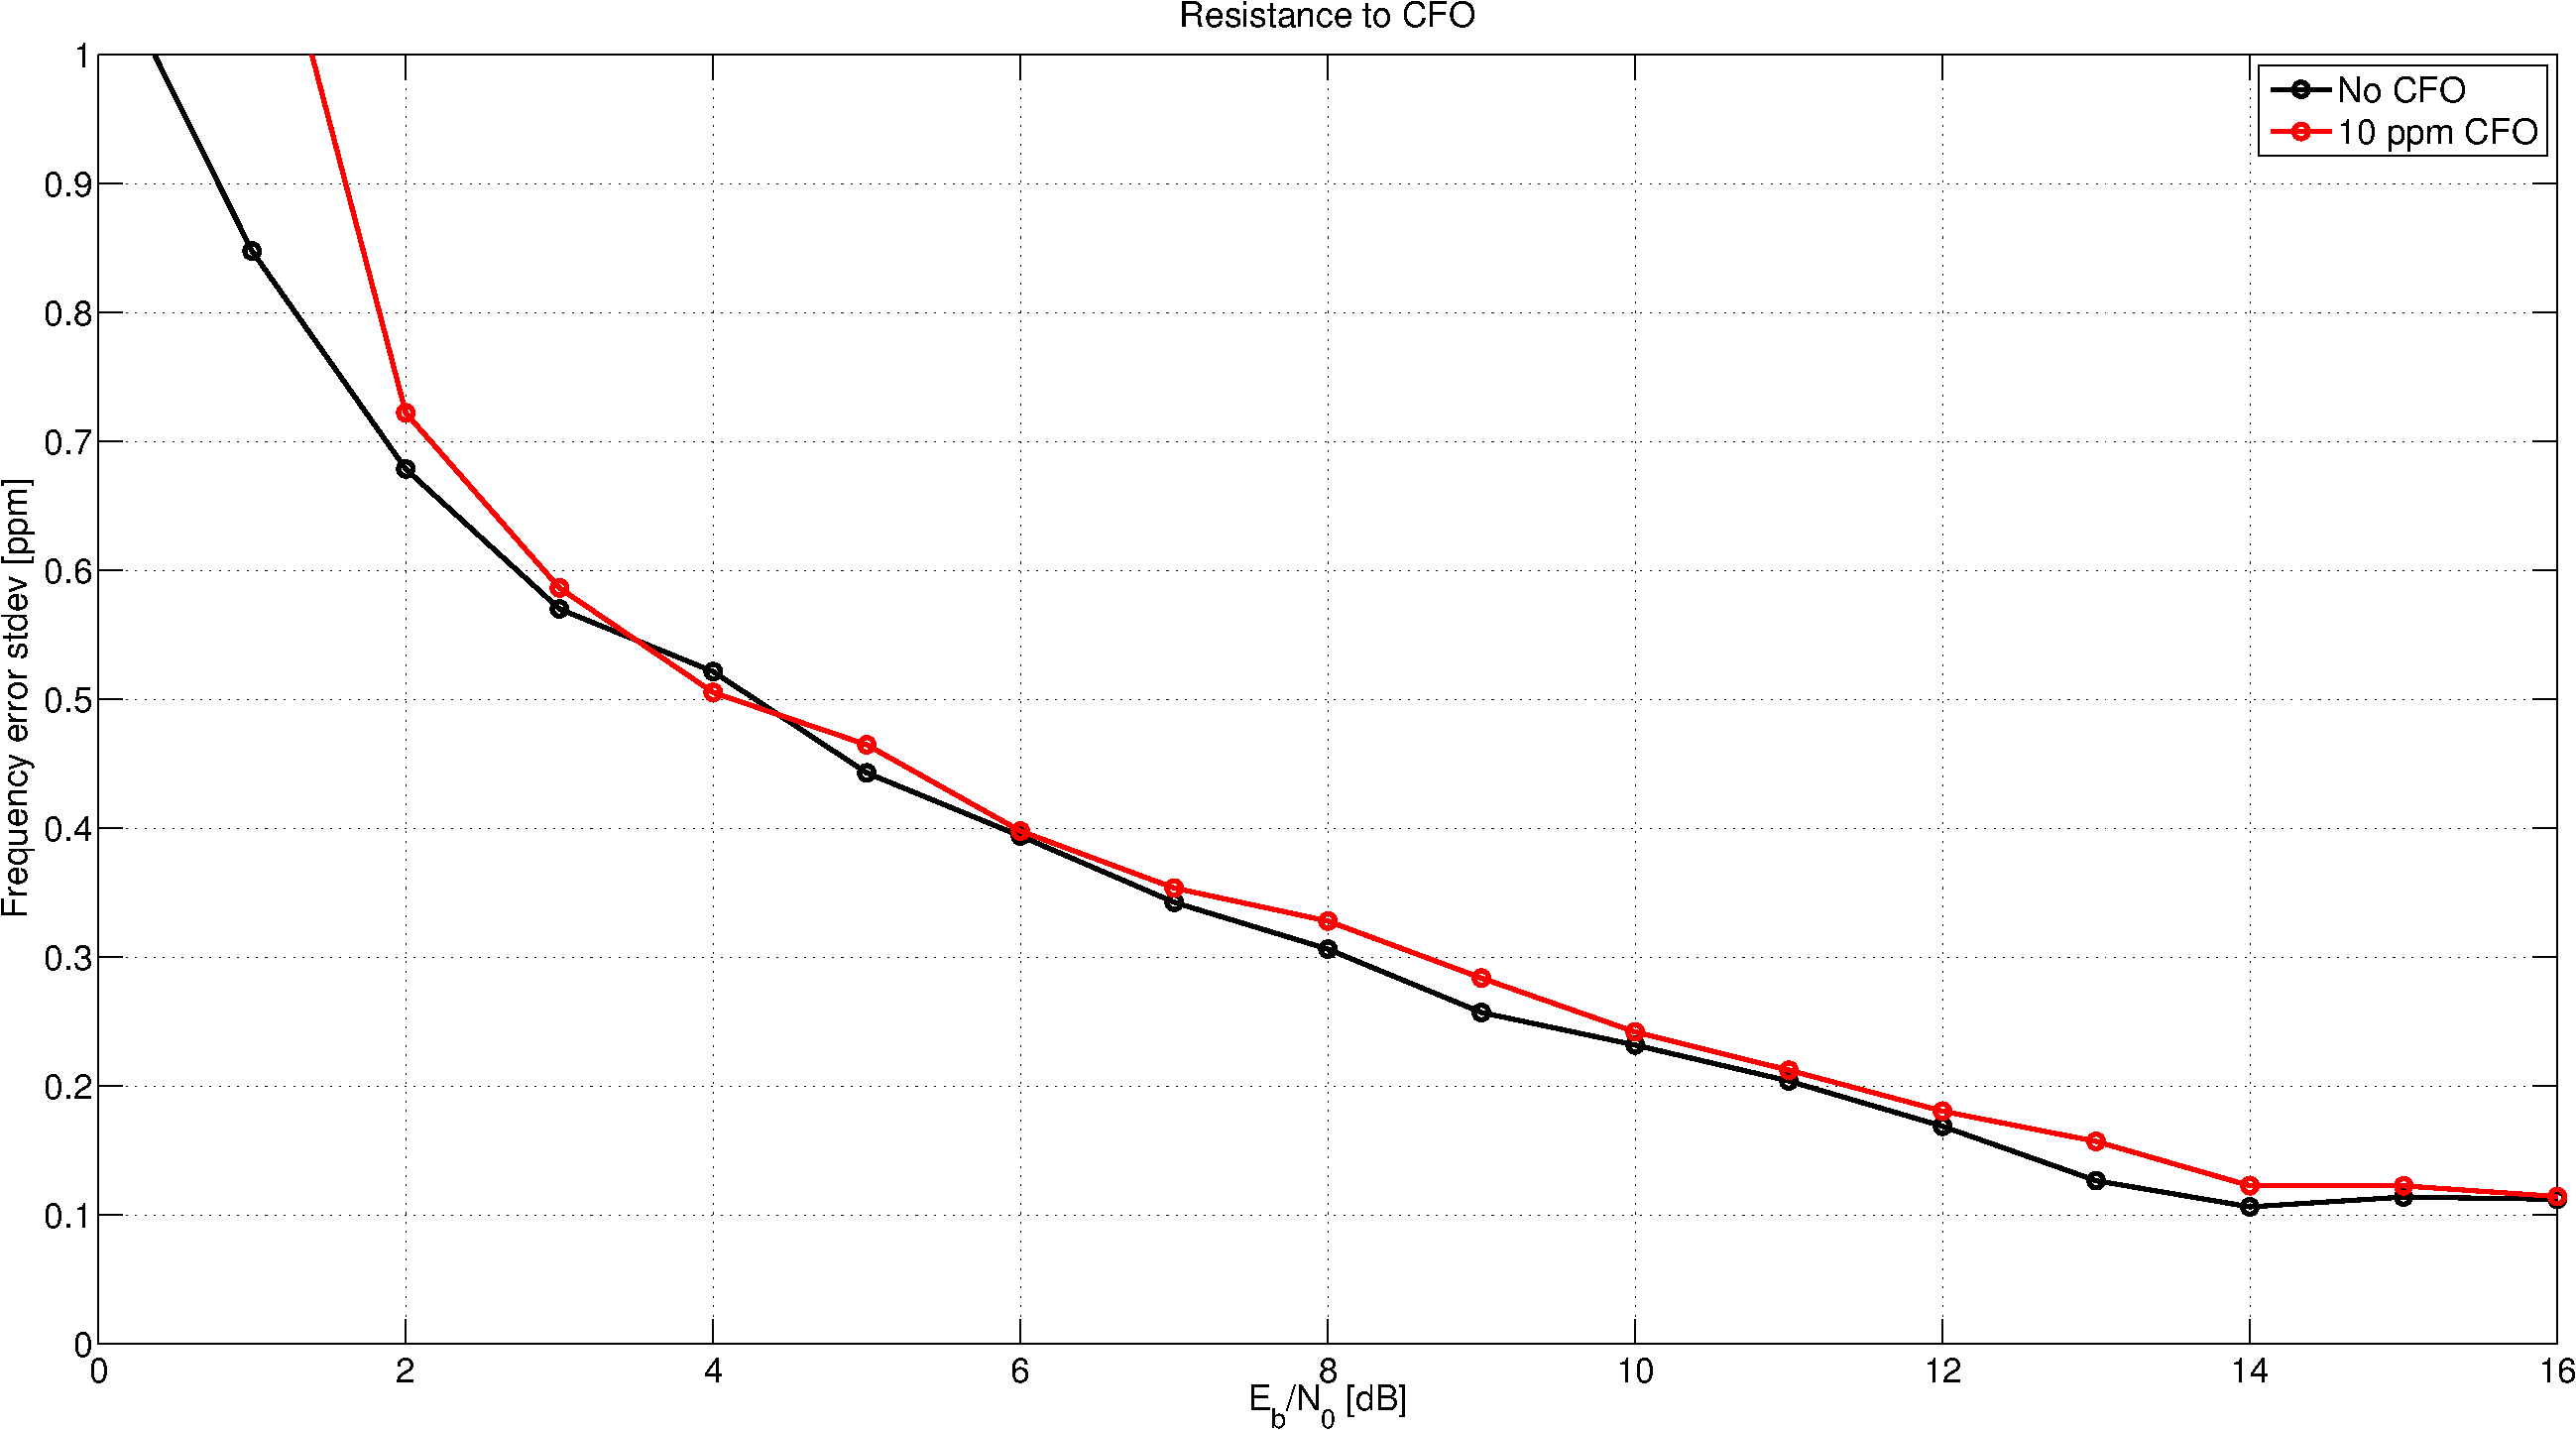
\includegraphics[width=\textwidth]{framecfocfo.pdf}
  \caption{Resistance of the CFO estimation to CFO.\label{fig:framecfocfo}}
\end{figure}
shows the resistance of the CFO estimation to CFO for 4-QAM modulation with $N = 40$ and $K=8$.

This shows that the ToA estimation is sufficient at realistic noise levels and standard CFO of \SI{10}{ppm}, but that frame interpolation is indeed needed to be able to correctly demodulate the incoming signal.
This is demonstrated in figure~\ref{fig:framecfoconst},
\begin{figure}
  \centering
  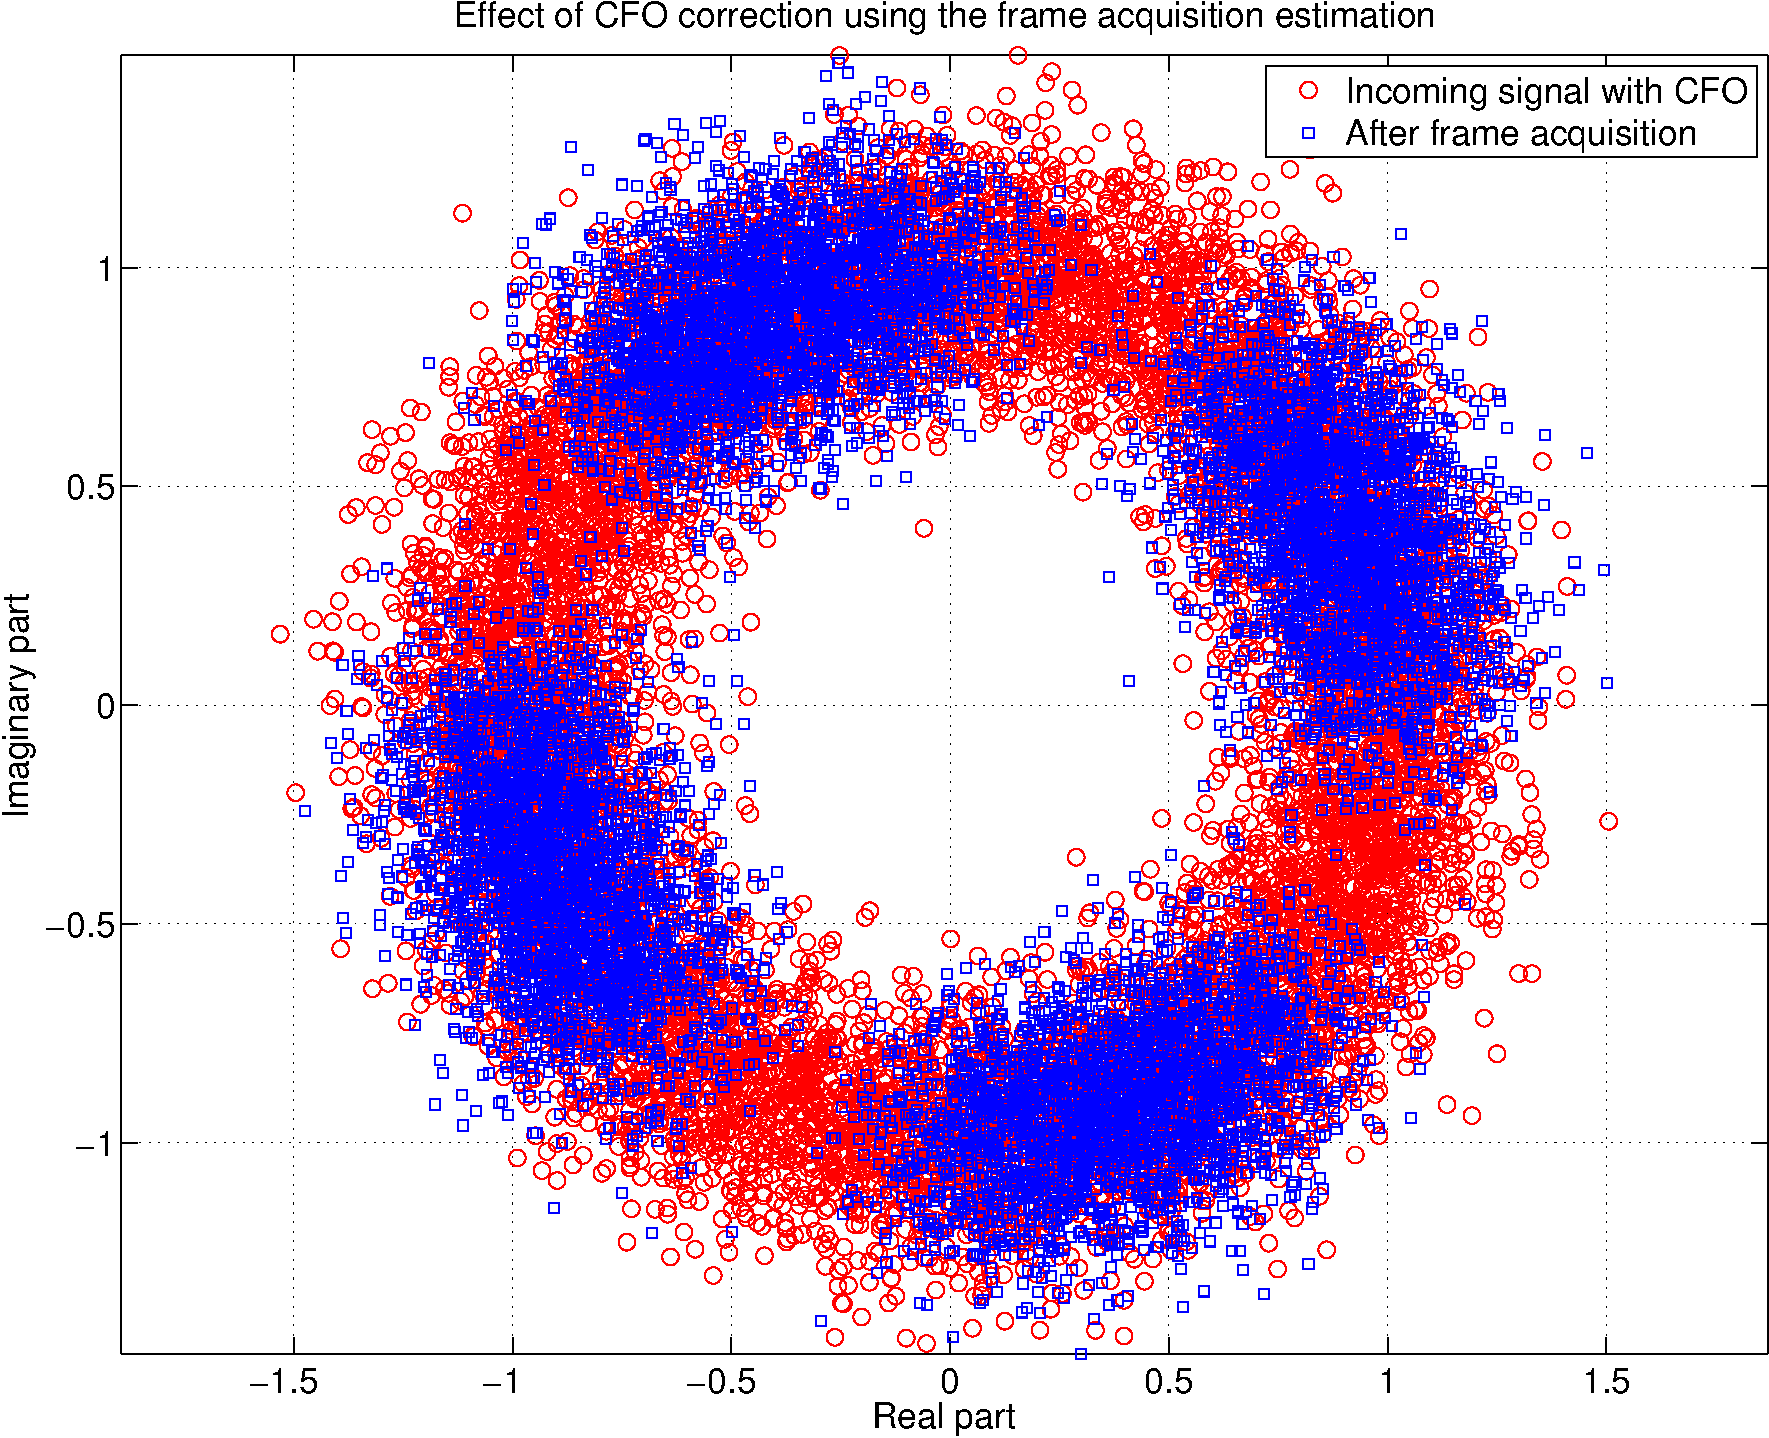
\includegraphics[width=.7\textwidth]{framecfoconstellation.pdf}
  \caption[Effect on the constellation of the frame acquisition]{Effect on the constellation of the frame acquisition (25 independent 512 bits blocks, remaining CFO = \SI{2.3}{ppm}).\label{fig:framecfoconst}}
\end{figure}
which shows that the remaining CFO still introduces a significant phase drift over the course of a single 512 bits block. However, frame acquisition is still able to compensate most of the synchronization error.


\subsection{Questions}
\subsubsection{Simulation}

\paragraph{Derive analytically the baseband model of the channel including the synchronisation errors.}
On figure~\ref{fig:mod},
\begin{figure}
  \centering
  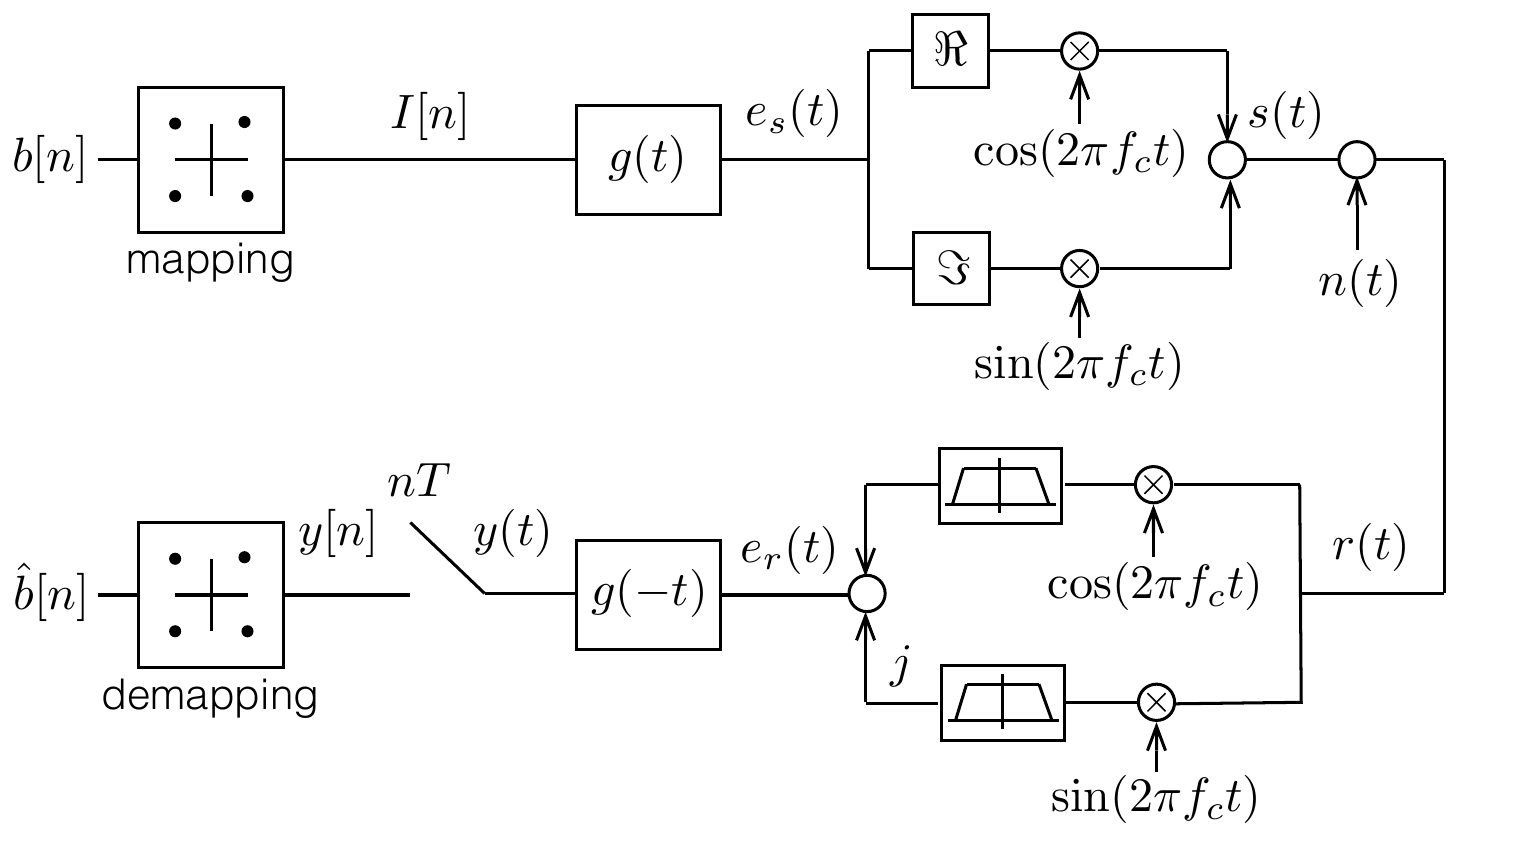
\includegraphics[width=\textwidth]{mod.png}
  \caption[Transceiver block diagram.]{Transceiver block diagram. [Source: course notes]\label{fig:mod}}
\end{figure}
let us now assume that the receiver's oscillator differs from the emitter's oscillator by $\Delta \omega$ in pulsation and by $\varphi$ in initial phase, and let us not consider the additive noise, which has already been covered previously.
We can write:
\begin{align*}
  r(t) = s(t) = &\real \{e_s(t)\} \cos(\omega_c t) + \imag \{e_s(t)\} \sin ( \omega_c t)\\
  e_r(t) = &\real \{e_s(t)\} \left [ \cos(\omega_c t)\cos((\omega_c + \Delta\omega) t + \varphi) + \cos(\omega_c t)\sin((\omega_c + \Delta\omega) t + \varphi) \right ] \\
  +j &\imag \{e_s(t)\} \left [ \sin(\omega_c t)\cos((\omega_c + \Delta\omega) t + \varphi) + \sin(\omega_c t)\sin((\omega_c + \Delta\omega) t + \varphi) \right ]
\end{align*}
By using simpson rules, and by removing the high frequency components which are eliminated by the low pass filters, we find:
\[
e_r(t) = \real\{e_s(t)\} \cos(\Delta \omega t + \varphi) - j\imag\{e_s(t)\} \sin(\Delta \omega t + \varphi)
\]
To obtain the baseband model of the channel, including CFO, we have to find $Z_{cfo}(t)$ such that:
\begin{align*}
  \real \left \{Z_{cfo}(t)\cdot e^{j\omega_c t} \right \} &= \real\{e_r(t)\} \cos(\omega_c t) - j \imag \{ e_r(t) \} \sin(\omega_c t)\\
  \Rightarrow Z_{cfo}(t) &= e_s(t)\cdot e^{j\Delta \omega t + \varphi}
\end{align*}
This means that the modulation/demodulation synchronization errors can be modeled in the baseband by multiplying the baseband signal by $e^{j\Delta \omega t + \varphi}$.

\paragraph{How do you separate the impact of the carrier phase drift and ISI due to the CFO in your simulation?}
To only measure the impact of the ISI introduced by the CFO, the CFO is perfectly corrected by hand after the filtering operation at the receiver.

\paragraph{How do you simulate the sampling time shift in practice?}The modulated message at the symbol frequency is first upsampled by a ratio $r_{os} = \frac{f_s}{f_m}$ before all the other operations.
At the receiver, after the filtering operation, the signal is downsampled.
During this downsampling operation, a fixed sampling time shift $t_0 = n \cdot T_s$ ($-\frac{r_{os}}{2} < n \leq \frac{r_{os}}{2}$, $n$ integer) can be introduced by shifting the indexes.

\paragraph{How do you select the simulated $E_{b}/N_{0}$ ratio?} $E_{b}/N_{0}$ should be small enough so that every block in the synchronization correction chain can converge correctly.
Else, if a block fails, for example Gardner compensation of the sample time shift, then every subsequent block will most likely fail as well, which means that the whole experience is useless.
However, $E_{b}/N_{0}$ should still be high enough so that it is realistic and it is possible to observe meaningful error rates.
A typical value is \SI{10}{\decibel}.

\paragraph{How do you select the lengths of the pilot and data sequences?} The pilot's length should be long enough to get a good estimation of the CFO and the ToA.
The length of a data sequence is selected to ensure a correct phase interpolation between two pilot sequences.
Furthermore, the pilot sequence length and repetition should be as small as those two considerations allow in order to maximize the channel throughput.

\subsubsection{Communication System}

\paragraph{In which order are the synchronisation effects estimated and compensated. Why?} First the sampling time shift is estimated and compensated with Gardner's algorithm, because frame and frequency acquisition can only work on a correctly sampled sequence, while Gardner's algorithm is robust to CFO.


\paragraph{Explain intuitively how the error is computed in the Gardner algorithm. Why is the
Gardner algorithm robust to CFO?} At step $n$, the time shift error is estimated by looking at the value of the signal between samples n and n-1. If there was a zero crossing, then the middle value should be zero or very small. The estimation of epsilon is then corrected by a term that is proportional to the value of this middle sample. The ``direction" of the correction is determined by the sign of the middle value and the direction of the zero crossing (upwards and negative value means the sampling is ``early", upwards and positive value means the sampling is ``late"; and vice-versa for downwards crossings).

\paragraph{Explain intuitively why the differential cross-correlator is better suited than the usual cross-correlator? Isn’t it interesting to start the summation at $k = 0$ (no time shift)?}
The differential cross-correlator first estimates the start time, and then the CFO. In doing so, it avoids an exhaustive 2D search which is computationally expensive. The alternative, a simple ToA ML estimation searches over a single parameter, but isn't robust to CFO.
It is not interesting to start the summation at $k = 0$ because the term $D_0[n]$ is given by:
\[
D_0[n] = \frac{1}{N}\cdot1\cdot\sum_{l=0}^{N-1} \left [ \big | I[n] \big | ^2 \big | a[l] \big | ^2 \right ]
\]
This shows that it only depends on the average power of the window, and so it couldn't provide additional information.

\paragraph{Are the frame and frequency acquisition algorithms optimal? If yes, give the optimisation criterion.}
The differential cross correlator algorithm isn't optimal because it doesn't optimize over $n$ and $\Delta \omega$ at once. However, it is sufficient for practical applications with CFO $\lesssim \SI{10}{ppm}$ and reasonable amounts of noise $\frac{E_b}{N_0} \gtrsim \SI{4}{\decibel}$
